\documentclass{beamer}
\usepackage{booktabs}
\usepackage{pdfpages}
\usepackage{mathtools}
\usepackage{enumerate}
\usepackage{multirow,tabularx}
\usepackage{booktabs}
\usepackage{pdfpages}
\usepackage{proof}
\usepackage{cancel}
\usepackage{chronology}
\usepackage{graphicx}
\usepackage{ulem}
\usepackage{amsmath}
\usepackage{amssymb}
\usepackage{color}
\usepackage{animate}
\usepackage{xr}

\PassOptionsToPackage{usenames,dvipsnames,svgnames}{xcolor}  
\usepackage{tikz}
\usepackage{tkz-graph}


\usepackage{wasysym}
\usepackage{proof}
\usepackage{cancel}
\usepackage{chronology}
\usepackage{graphicx}
\usepackage{ulem}
\usepackage{amsmath}
\usepackage{amssymb}
\usepackage{color}
\usepackage{xcolor}
\usepackage{soul}
%\usepackage{pstricks}
\setbeamertemplate{navigation symbols}{}

\newcommand{\norm}[1]{\left\lVert#1\right\rVert}
\newcommand{\el}{$\mathcal{EL}^{++}$}
\renewcommand{\Re}{\mathbb{R}}
\newcommand{\BigO}[1]{\ensuremath{\operatorname{O}\bigl(#1\bigr)}}
\newcommand{\myul}[2][blue]{\sethlcolor{#1}\hl{#2}\setulcolor{black}}

\newcommand<>{\cunderline}[3]{\only<#1>{#3}\only<#2>{\underline{#3}}}
\newcommand<>{\cem}[3]{\only<#1>{#3}\only<#2>{\ul{#3}}}
\newcommand<>{\cgray}[3]{\only<#1>{#3}\only<#2>{\textcolor{gray}{#3}}}
\newcommand<>{\colorize}[4]{\only<#1>{#4}\only<#2>{\textcolor{#3}{#4}}}

\setbeamertemplate{navigation symbols}{\insertslidenavigationsymbol}
%\setbeamertemplate{navigation symbols}{}
% \addtobeamertemplate{navigation symbols}{}{%
%     \usebeamerfont{footline}%
%     \usebeamercolor[fg]{footline}%
%     \hspace{1em}%
%     \insertframenumber/\inserttotalframenumber
% }

\mode<presentation>
{
\usecolortheme{crane}
%\useoutertheme{split}

\expandafter\def\expandafter\insertshorttitle\expandafter{%
  \insertshorttitle\hfill%
  \insertframenumber\,/\,\inserttotalframenumber}

\usefonttheme[onlysmall]{structurebold}
}
\renewcommand{\em}{\itshape}
\usepackage{pifont}
\definecolor{purple}{rgb}{1,0,1}
\definecolor{dred}{rgb}{0.7,0,0}
\definecolor{myred}{rgb}{1,0,0}
\definecolor{dblue}{rgb}{0,0,0.7}
\definecolor{dgreen}{rgb}{0,0.5,0}
\definecolor{myyellow}{rgb}{1,1,0}
\newcommand{\parents}[1]{parents(#1)}
\setbeamertemplate{itemize item}[ball]


% \mode<presentation>
% {
% \useinnertheme[shadow=true]{rounded}
% \useoutertheme{infolines}
% \usecolortheme{dove}
% \setbeamerfont{block title}{size={}}
% }

\title[Bio-Ontologies]{Semantic similarity and machine learning with ontologies}

\author{Robert Hoehndorf and Maxat Kulmanov}


\date{}

\begin{document}

\begin{frame}
  \titlepage
\end{frame}

\section{Embedding ontologies}

\begin{frame}
  \frametitle{Embedding ontologies: approaches}
  \begin{itemize}
  \item syntactic: treat axioms as ``sentences'' using language models
  \item graph-based: treat ontologies as graphs (like in semantic similarity)
  \item model-theoretic: encode model-theoretic semantics in optimization
  \end{itemize}
\end{frame}

\subsection{Syntactic approaches}

\begin{frame}
  \frametitle{Ontologies: axioms, not graphs!}
    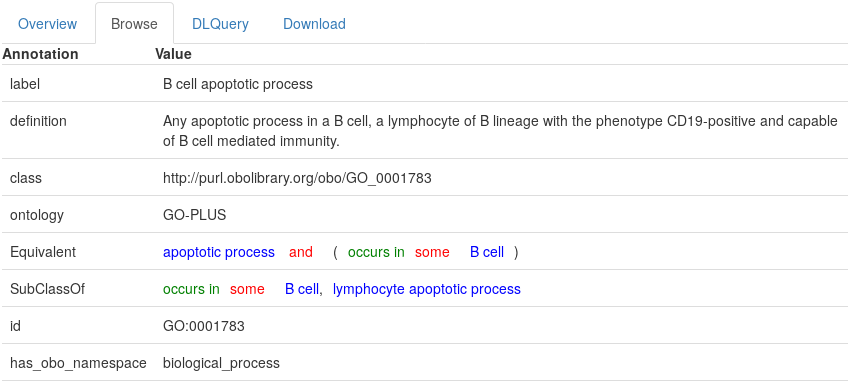
\includegraphics[width=1\textwidth]{bcellapoptosis.png}
\end{frame}

\begin{frame}
  \frametitle{Ontologies: axioms, not graphs!}
  Gene Ontology:
  \begin{itemize}
  \item {\tt behavior DisjointWith: 'developmental process'}
  \item {\tt behavior SubclassOf: only-in-taxon some metazoa}
  \item {\tt 'cell proliferation' DisjointWith: in-taxon some fungi}
  \item {\tt 'cell growth' EquivalentTo: growth and ('results in
      growth of' some cell)}
  \item ...
  \end{itemize}
\end{frame}

% \begin{frame}
%   \frametitle{Ontologies: axioms, not graphs!}
%   \begin{itemize}
%   \item converting ontologies to graphs
%     \begin{itemize}
%     \item loses information
%     \end{itemize}
%   \item relations between ontologies
%   \end{itemize}
% \end{frame}

\begin{frame}
  \frametitle{Ontology embeddings}
  \begin{definition}
    Let $O = (\Sigma = (C, R, I); ax; \vdash)$ be an ontology with a set of
    classes $C$, a set of relations $R$, a set of instances $I$, a set
    of axioms $ax$ and an inference relation $\vdash$. An ontology
    embedding is a function $f_\eta : C \cup R \cup I \mapsto
    \Re^n$ (or $\Sigma(O) \mapsto \Re^n$ (subject to certain constraints).
  \end{definition}
  \pause For example, we can use co-occurrence within $ax^\vdash$ to
  constrain the embedding function, where the constraints on
  co-occurrence are formulated using the Word2Vec skipgram model.
\end{frame}

\begin{frame}
  \frametitle{Onto2Vec}
  \centerline{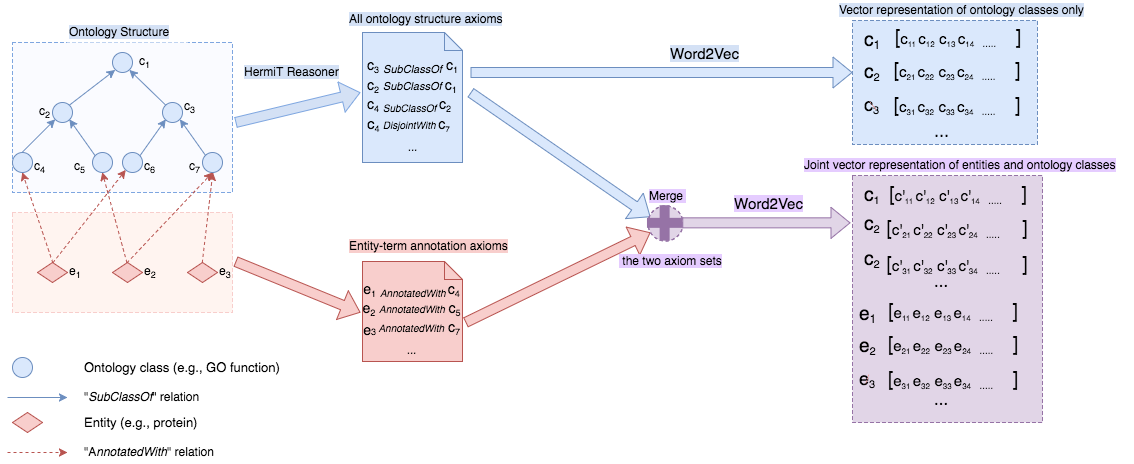
\includegraphics[width=\textwidth]{onto2vecflow.png}}
\end{frame}

\begin{frame}
  \frametitle{Word2Vec}
  Maximize:
  \begin{equation}
    \frac{1}{N} \sum_{n=1}^{N} \sum_{-c\leq j \leq c, j\not=
      0} \log p(w_{n+j}|w_n)
  \end{equation}
  with
  \begin{equation}
    p(w_o | w_i) = \frac{\exp({v'_{w_o}}^T v_{w_i})}{\sum_{w=1}^{W}
      \exp({v'_{w}}^T v_{w_i})}
  \end{equation}
  (at least conceptually; different strategies are used to approximate Eqn. 2)
\end{frame}

% \begin{frame}
%   \frametitle{Word2Vec}
%   \centerline{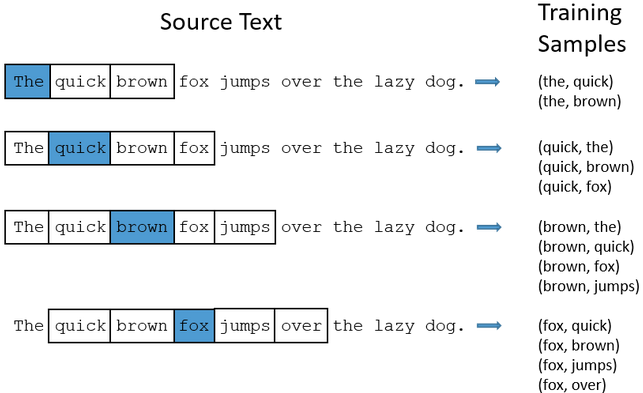
\includegraphics[width=\textwidth]{word2vec-example.png}}
% \end{frame}

\begin{frame}
  \frametitle{Predicting PPIs: trainable similarity measures}
  \centerline{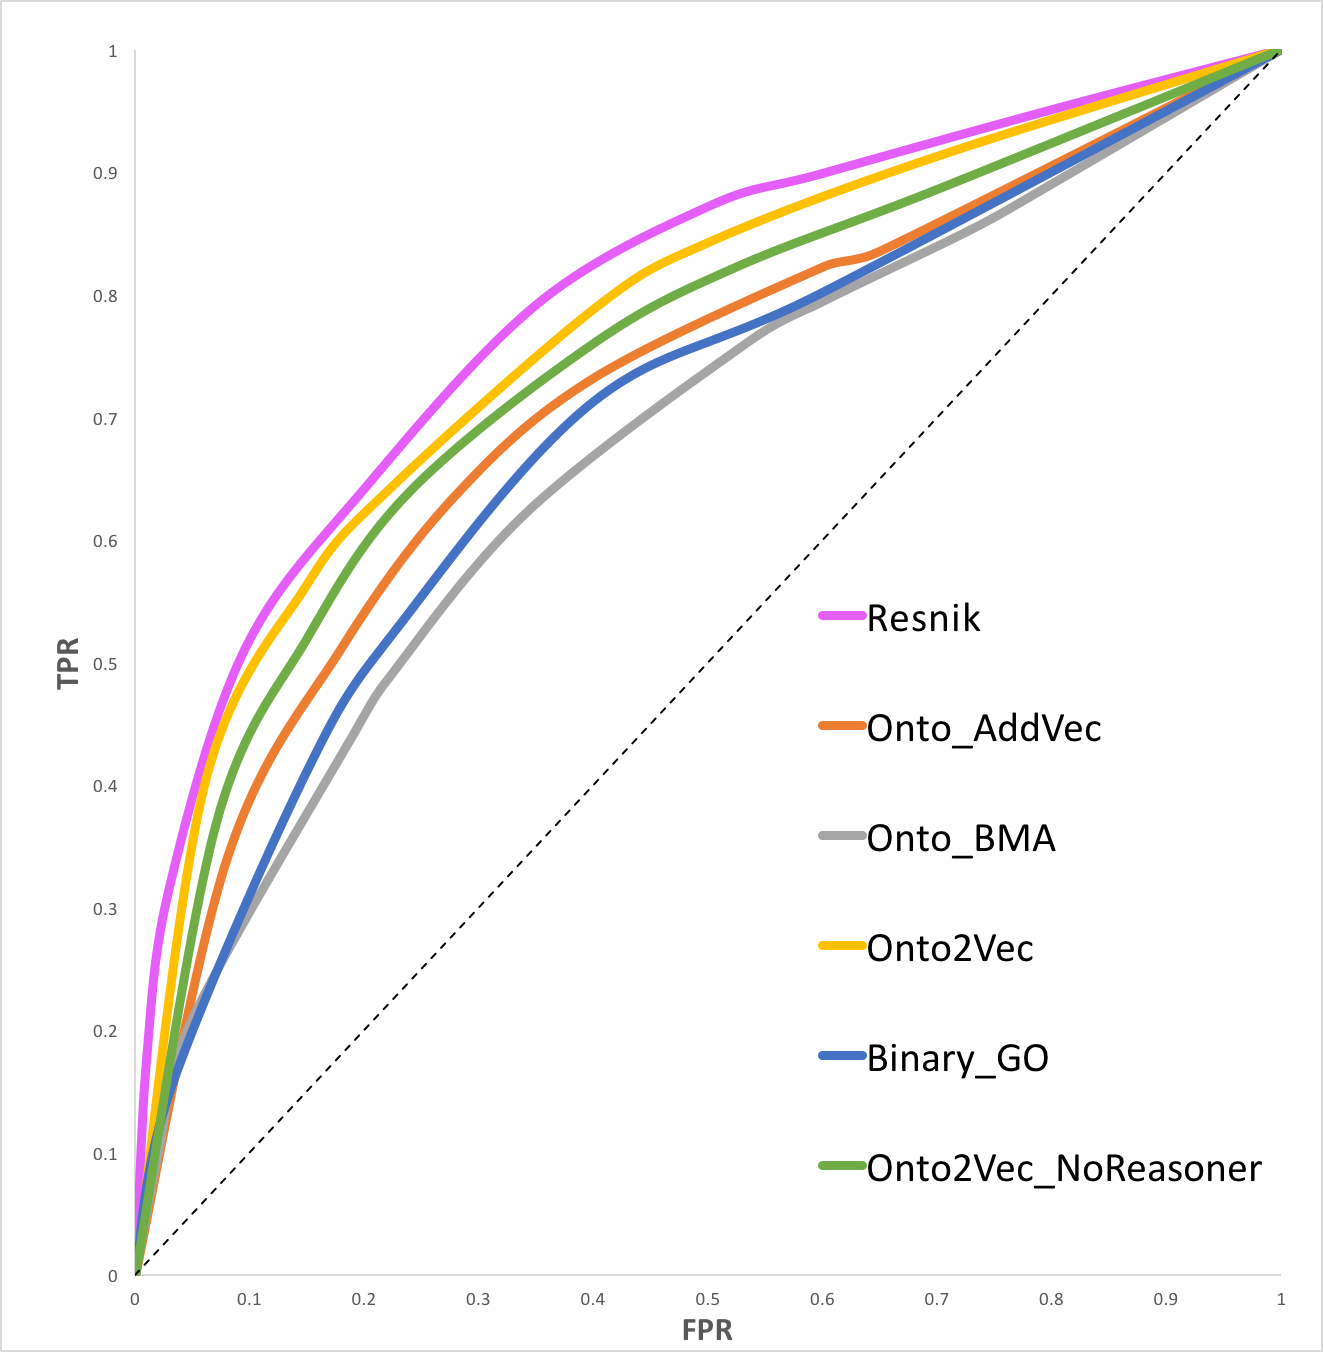
\includegraphics[width=.45\textwidth]{YSTUnsuper1.png}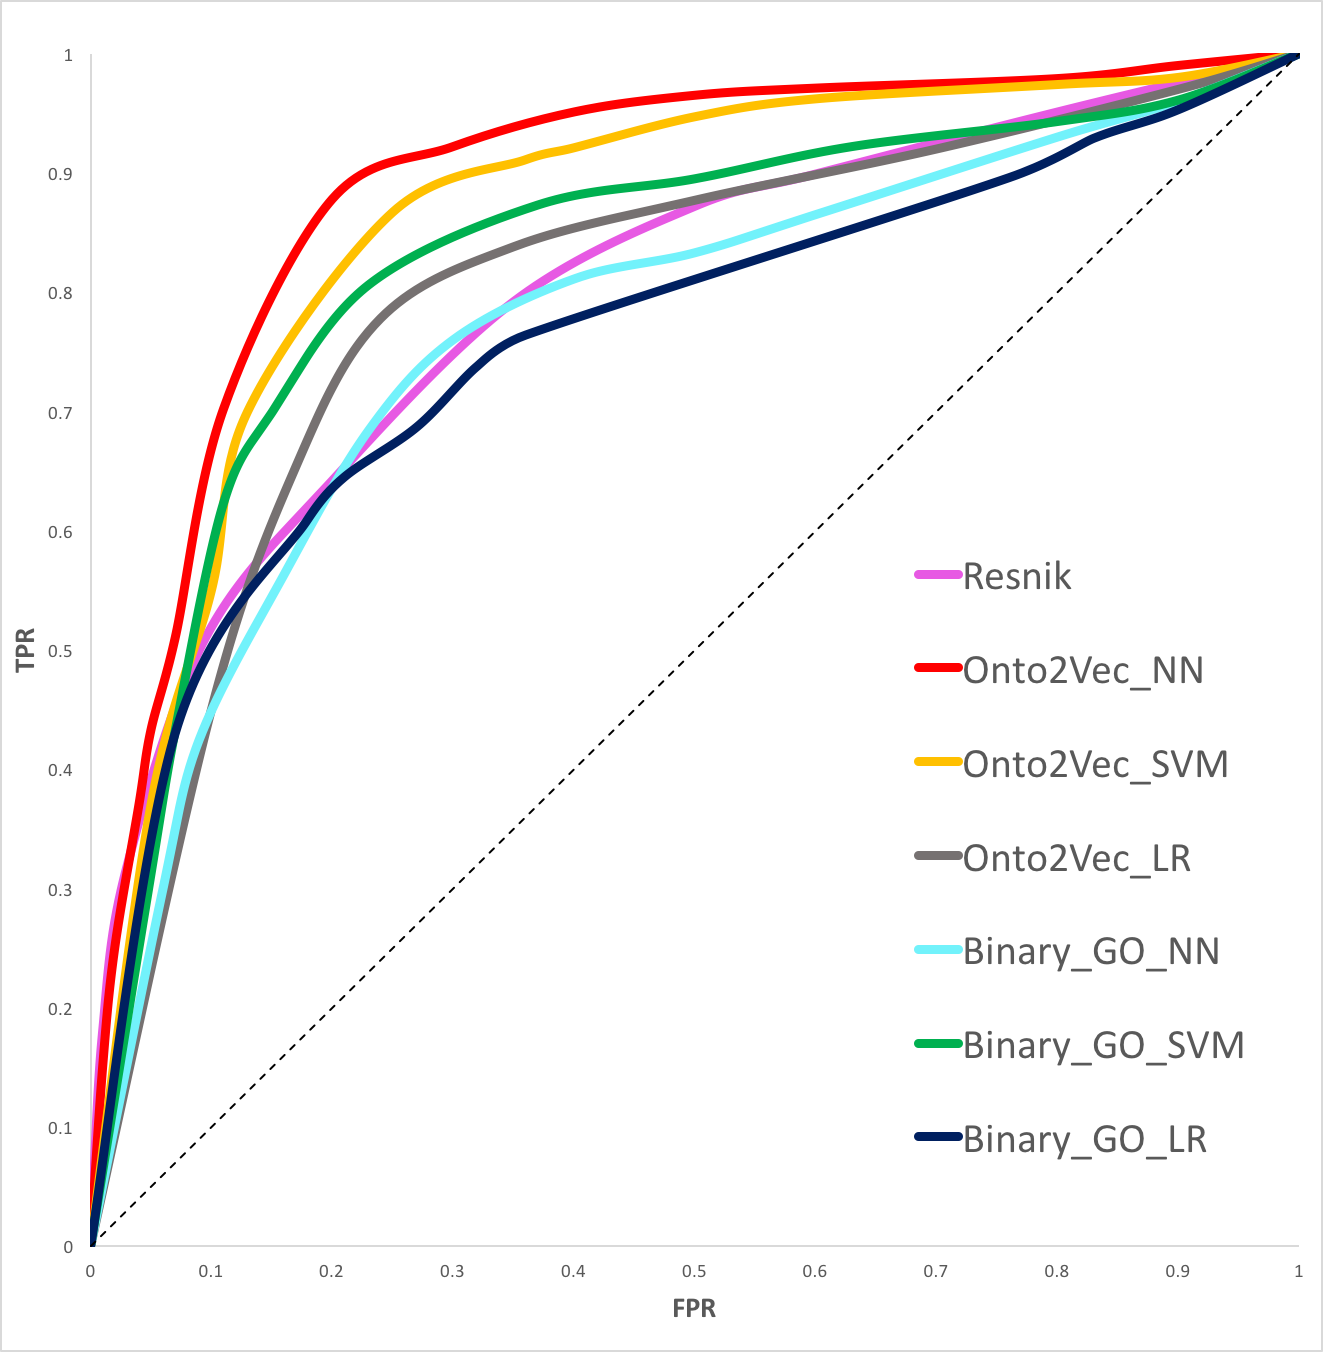
\includegraphics[width=.45\textwidth]{YstUnsup2.png}}

   {\tiny Smaili et al. Onto2Vec: joint vector-based representation of
     biological entities and their ontology-based annotations.}
\end{frame}

\begin{frame}
  \frametitle{Visualizing embeddings}
  \centerline{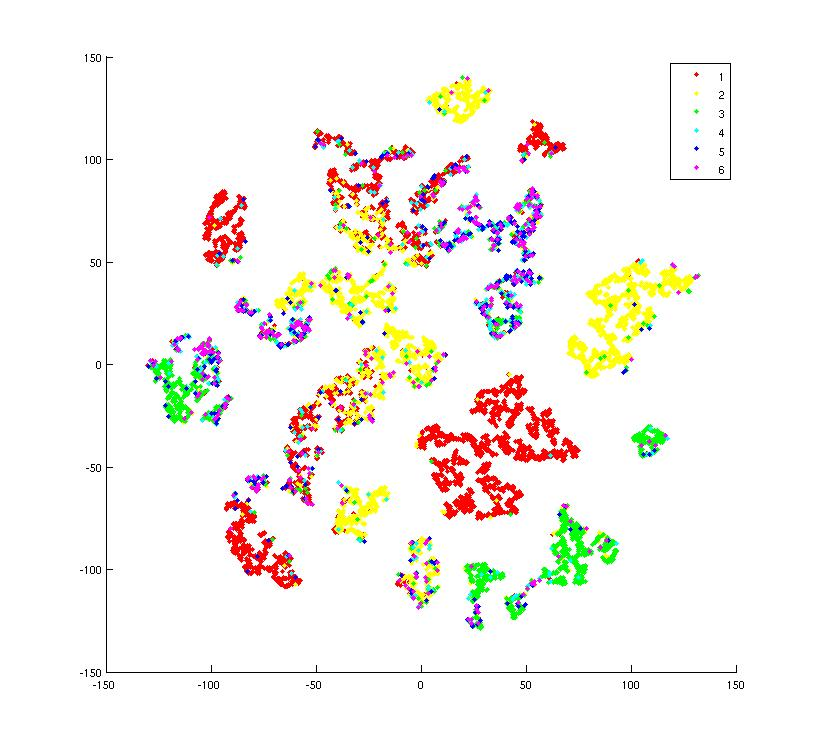
\includegraphics[width=.9\textwidth]{updtsne.jpg}}
\end{frame}

\begin{frame}
  \frametitle{Combination with text}
  \begin{itemize}
  \item ontologies contain more than axioms:
    \begin{itemize}
    \item labels, synonyms, definitions, authors, etc.
    \end{itemize}
  \item Description Logic axioms != natural language
  \item transfer learning: learn on one domain/task, apply to another
    \begin{itemize}
    \item e.g.: learn on literature, apply to ontologies
    \item words have ``meaning'' in literature, Description Logic
      symbols have ``meaning'' in ontology axioms
    \end{itemize}
  \item Ontologies Plus Annotations 2 Vec (OPA2Vec) combines both
  \end{itemize}
\end{frame}

\begin{frame}
  \frametitle{Ontologies Plus Annotations 2 Vec}
  \centerline{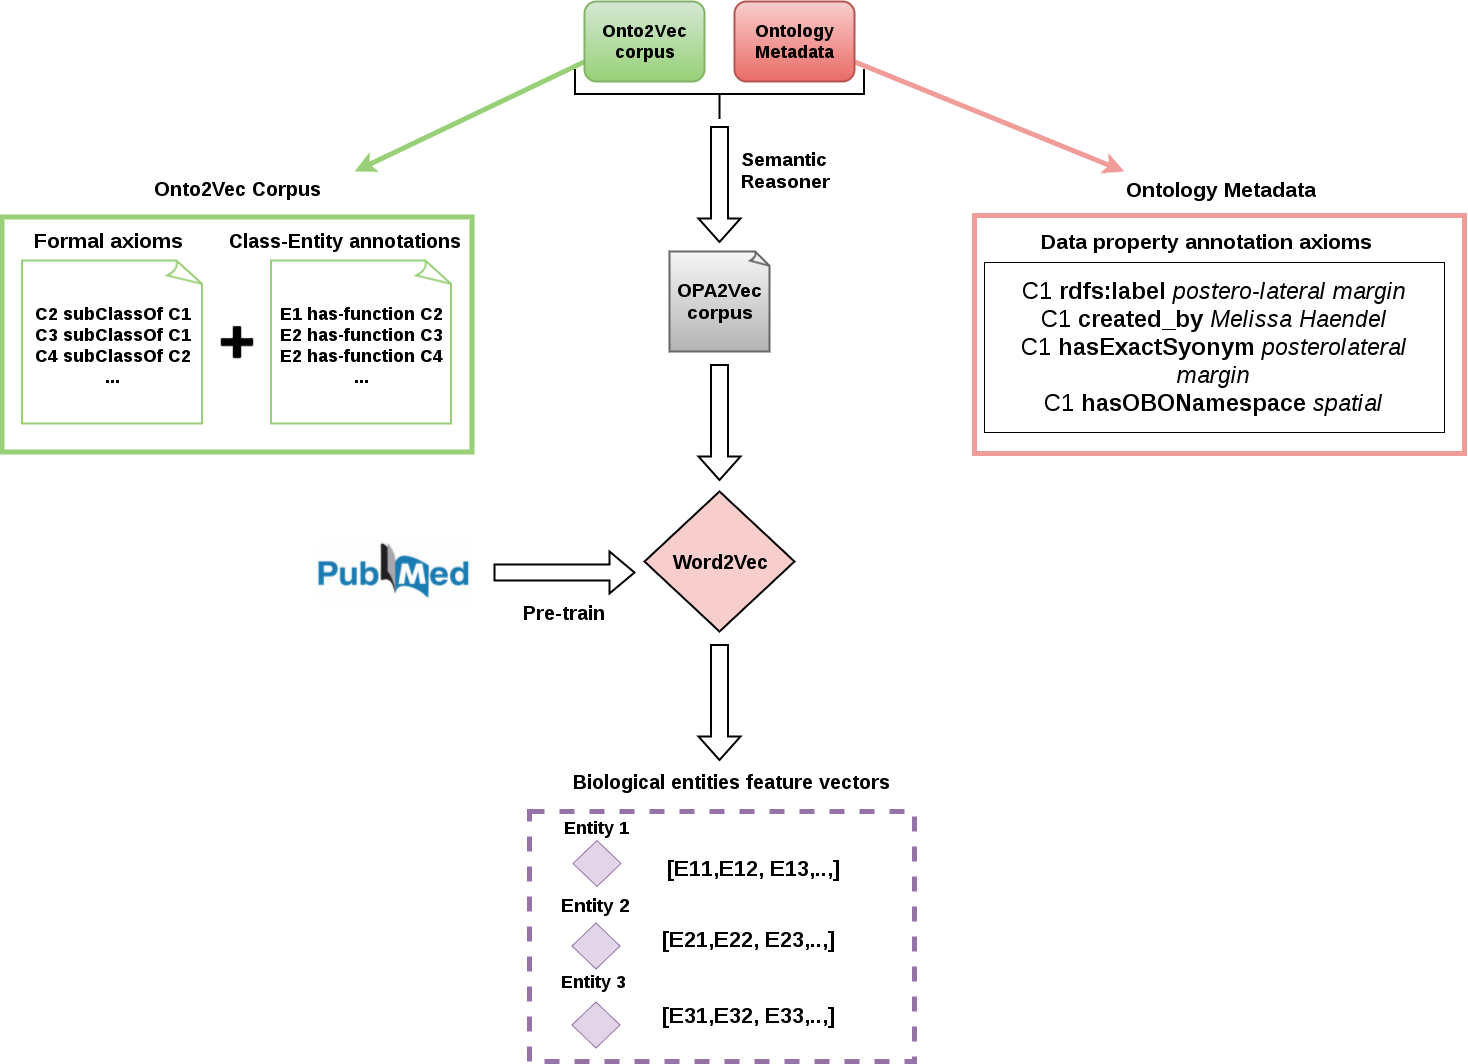
\includegraphics[width=1\textwidth]{opaworkflow16.png}}
\end{frame}

\begin{frame}
  \frametitle{Axioms contribute to prediction tasks: GO and GO-PLUS}
    % \processtable
    % \caption{AUC values of ROC curves for PPI prediction for
    %   GO-Plus and GO using Onto2Vec (cosine similiarity) and
    %   Onto2Vec-NN (neural network).\label{Tab:GOplus}}
    { \begin{tabularx}{\columnwidth}{XXXXXXX}\toprule & {}& {} &
                                                                 Human & Yeast & Arabidopsis\\\midrule
        $GO\_Onto2Vec$ & {} &{}& 0.7660 & 0.7701 & 0.7559 \\
        $GO\_Onto2Vec\_NN$ & {} & {}& 0.8779& 0.8711 & 0.8364 \\
        $GO\_plus\_Onto2Vec$ & {} & {}& 0.7880& 0.7943 & 0.7889 \\
        $GO\_plus\_Onto2Vec\_NN$ &{} & {}& \textbf{0.9021}&\textbf{0.8937} & \textbf{0.8834}\\
        \hline
      \end{tabularx}}{}
\end{frame}

\begin{frame}
  \frametitle{Evaluating individual axioms}
%  Testing how much each ontologies' axioms contribute to predictions:
%  \begin{resizebox}{\textwidth}{!}{
  Testing how much each ontologies' axioms contribute to predictions:
  \tiny
      \begin{tabularx}{\linewidth}{X|XX|XX}
        \toprule
        {} & \multicolumn{2}{c}{\textbf{Human}} & \multicolumn{2}{c}{\textbf{Arabidopsis}}\\
        \midrule
        {} & \textbf{Onto2Vec}&\textbf{Onto2Vec\_NN} &\textbf{Onto2Vec}&\textbf{Onto2Vec\_NN} \\
        \midrule
        GO (Baseline) &0.7660 &0.8779  & 0.7559 & 0.8364 \\
        ChEBI &0.7899\textcolor{blue}{(+0.0239)}& 0.8914\textcolor{blue}{(+0.0135)}  & 0.7703\textcolor{blue}{(+0.0144)}& 0.8518\textcolor{blue}{(+0.0154)} \\
        PO &0.7752\textcolor{blue}{(+0.0092)} & 0.8776\textcolor{red}{(-0.0003)} & 0.7671\textcolor{blue}{(+0.0112)} & 0.8469\textcolor{blue}{(+0.0105)}\\
        CL & 0.7743\textcolor{blue}{(+0.0083)} & 0.8810\textcolor{blue}{(+0.0031)} & 0.7612\textcolor{blue}{(+0.0053)}& 0.8371\textcolor{blue}{(+0.0007)}\\
        PATO & 0.7657\textcolor{red}{(-0.0003)} & 0.8768\textcolor{red}{(-0.0011)} & 0.7563\textcolor{blue}{(+0.0004)} & 0.8380\textcolor{blue}{(+0.0016)}\\
      \end{tabularx}
%    }
%  \centerline{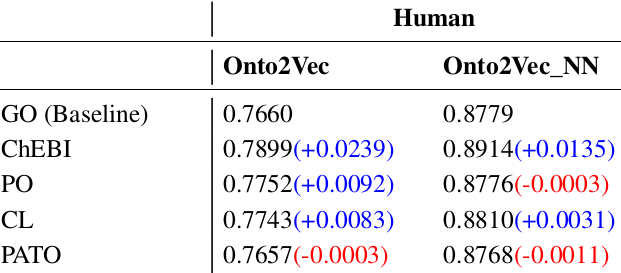
\includegraphics[width=1\textwidth]{pato-eval1.png}}
\end{frame}

\begin{frame}
  \frametitle{Evaluating definitions}
  Testing how much each ontologies' annotation properties contribute to predictions:
  \tiny
      \begin{tabularx}{\linewidth}{X|XX|XX}
        \toprule
        {} & \multicolumn{2}{c}{\textbf{Human}} & \multicolumn{2}{c}{\textbf{Arabidopsis}}\\
        \midrule
        {} & \textbf{Onto2Vec}&\textbf{Onto2Vec\_NN} &\textbf{Onto2Vec}&\textbf{Onto2Vec\_NN} \\
        \midrule
        GO (Baseline)&0.8727 &0.9033  & 0.8613 & 0.8903 \\
        ChEBI & 0.8571\textcolor{red}{(-0.0156)} &0.8801\textcolor{red}{(-0.0232)} &0.8601\textcolor{red}{(-0.0012)}& 0.8880\textcolor{red}{(-0.0023)}\\
        PO & 0.8680\textcolor{red}{(-0.0047)}&0.8824\textcolor{red}{(-0.0209)} & 0.8632\textcolor{blue}{(+0.0019)} & 0.8908\textcolor{blue}{(+0.0005)}\\
        CL & 0.8811\textcolor{blue}{(+0.0084)}&0.9037\textcolor{blue}{(+0.0004)}  & 0.8614\textcolor{blue}{(+0.0001)} & 0.8899\textcolor{red}{(-0.0004)}\\
        PATO & 0.8562\textcolor{red}{(-0.0165)}& 0.8711\textcolor{red}{(-0.0322)} & 0.8544\textcolor{red}{(-0.0069)}& 0.8860\textcolor{red}{(-0.0043)} \\
      \end{tabularx}
%  \centerline{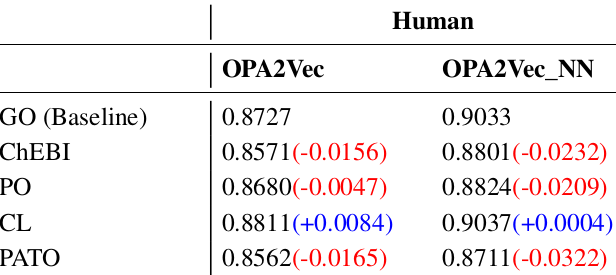
\includegraphics[width=1\textwidth]{pato-eval2.png}}
\end{frame}

\begin{frame}
  \frametitle{OPA2Vec}
  \begin{itemize}
  \item \url{https://github.com/bio-ontology-research-group/opa2vec}
  \item command line tool
    \begin{itemize}
    \item input: OWL ontology, set of entities with annotations/associations
    \item output: vectors for each class and entity
    \end{itemize}
  \item includes Elk and HermiT
  \item limitations: word-based
    \begin{itemize}
    \item completely ignores any semantics!
    \end{itemize}
  \end{itemize}
\end{frame}

\subsection{Graph-based methods}

% \begin{frame}
%   \frametitle{Graph-based Learning}
%   \centerline{\includegraphics[height=.8\textheight]{instances.png}}
%   {\tiny From Harispe et al., Semantic Similarity From Natural
%     Language And Ontology Analysis, 2015.}
% \end{frame}

\begin{frame}
  \frametitle{How to measure similarity?}
  \begin{itemize}
  \item Shortest Path
    \begin{itemize}
    \item applicable to arbitrary ``knowledge graphs''
    \item does not capture similarity well over all edge types, e.g.,
      {\em disjointWith}, {\em differentFrom}, {\em opposite-of}, etc.
    \end{itemize}
  \item Random Walk
    \begin{itemize}
    \item with or without restart
    \item iterated
    \item does not consider edge labels $\Rightarrow$ captures only
      adjacency of nodes
    \item scores whole graph with {\em probability} of being in a
      state
    \item can take multiple seed nodes
      \begin{itemize}
      \item can be used to find disease genes
      \end{itemize}
    \end{itemize}
  \end{itemize}
\end{frame}


\begin{frame}
  \frametitle{Graph-based learning}
  \begin{itemize}
  \item feature learning on graphs
    \pause
  \item e.g., iterated, edge-labeled random walk
    \begin{itemize}
      % \item over instances and classes
    \item walks form {\em sentences}
    \item sentences form a {\em corpus}
    \item feature learning on corpus through Word2Vec (or factorization
      of co-occurrence matrix)
    \item RDF2Vec:
      \url{http://data.dws.informatik.uni-mannheim.de/rdf2vec/}
    \item with support for reasoning over ontologies:
      \url{https://github.com/bio-ontology-research-group/walking-rdf-and-owl}
    \end{itemize}
    \pause
  \item Translational knowledge graph embeddings: TransE, TransR, TransE, HolE, etc.
    \begin{itemize}
    \item analogy- or translation-based
    \item \url{https://github.com/SmartDataAnalytics/PyKEEN}
    \end{itemize}
    \pause
  \item Graph Convolution Neural Networks (not discussed here)
  \end{itemize}
\end{frame}

% \begin{frame}
%   \frametitle{Graph-based learning}
%   \begin{itemize}
%   \item graph-representation of the ontology
%     \begin{itemize}
%     \item taxonomy
%     \item axioms
%     \item instances (using an {\tt instance-of} edge)
%     \end{itemize}
%   \item learning with graphs:
%     \begin{itemize}
%     \item random walks (and Word2Vec)
%     \item translation embeddings
%     \end{itemize}
%   \end{itemize}
% \end{frame}

\begin{frame}
  \frametitle{Graph embeddings}
  \begin{definition}
    Let $KG = (V, E, L; \vdash)$ be an ontology graph with a set of
    vertices $V$, a set of edges $E \subseteq V \times V$, a label
    function $L: V \cup E \mapsto Lab$ that assigns labels from a set
    of labels $Lab$ to vertices and edges, and an inference relation
    $\vdash$. An ontology graph embedding is a function
    $f_\eta : L(V) \cup L(E) \mapsto \mathbf{R}^n$.
  \end{definition}
  \pause
  \begin{itemize}
  \item key idea: preserve {\em some} structure of the graph in
    $\Re^n$ (under operations in $\Re^n$)
  \item $\Re^n$ enables {\em new} operations (such as many similarity
    measures)
  \item useful as {\em feature} vectors
  \end{itemize}
\end{frame}

\begin{frame}
  \frametitle{Random walks}
  \begin{columns}
    \begin{column}{.6\textwidth}
      \resizebox{1\textwidth}{!}{%
        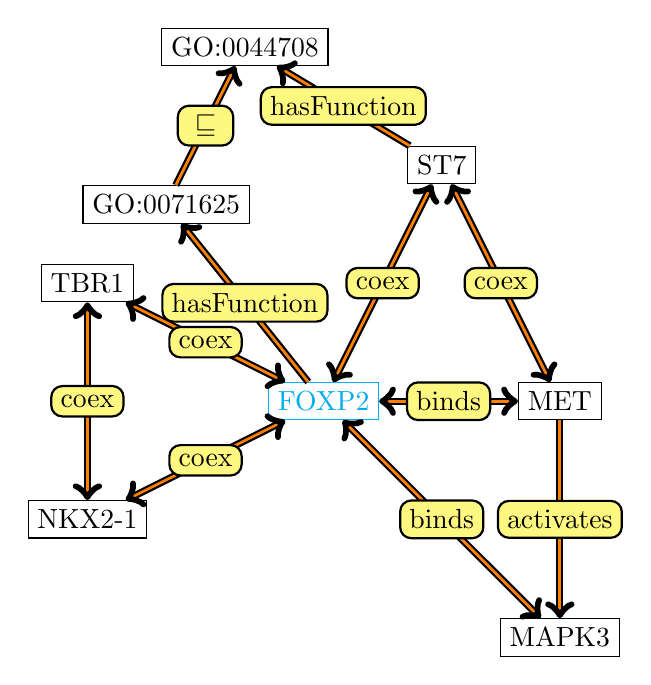
\begin{tikzpicture}
%          \SetUpEdge[lw = 1pt, color = black]
          \GraphInit[vstyle=Shade]
          \tikzset{
            LabelStyle/.style = { rectangle, rounded corners, draw,
              minimum width = 2em, fill = yellow!50,
              text = black },
            VertexStyle/.append style = { inner sep=5pt,
              font = \Large\bfseries},
            EdgeStyle/.append style = {->} }
          
          \SetGraphUnit{5}
          % \tikzset{VertexStyle/.append style={fill}}
          % \tikzset{EdgeStyle/.style={->}}
          \node[draw, color=cyan] (FOXP2) at (0,0) {FOXP2};
          \node[draw] (MET) at (3,0) {MET};
          \node[draw] (ST7) at (1.5,3) {ST7};
          \node[draw] (MAPK3) at (3,-3) {MAPK3};
          \node[draw] (GO0071625) at (-2,2.5) {GO:0071625};
          \node[draw] (GO0044708) at (-1,4.5) {GO:0044708};
          \node[draw] (TBR1) at (-3,1.5) {TBR1};
          \node[draw] (NKX2-1) at (-3,-1.5) {NKX2-1};
          \begin{scope}[/tikz/handle active characters in nodes=false]
          \Edge[label=activates](MET)(MAPK3)
          \Edge[label=hasFunction](FOXP2)(GO0071625)
          \Edge[label=hasFunction](ST7)(GO0044708)
          \Edge[label=$\sqsubseteq$](GO0071625)(GO0044708)

          \tikzset{EdgeStyle/.append style={<->}}
          \Edge[label=binds](FOXP2)(MET)
          \Edge[label=binds](FOXP2)(MAPK3)
          \Edge[label=coex](FOXP2)(TBR1)
          \Edge[label=coex](FOXP2)(NKX2-1)
          \Edge[label=coex](FOXP2)(ST7)
          \Edge[label=coex](MET)(ST7)
          \Edge[label=coex](NKX2-1)(TBR1)
          \end{scope}
          % \tikzset{EdgeStyle/.style={->}}
          % \Edge[label=hf](FOXP2)(GO0044708)
          % \draw[label=binds] (FOXP2) to (MET);
          % \Edge[label=binds](FOXP2)(MET)
          % \Edge[label=activates](MET)(MAPK3)
          % \Edge[label=coexpressed-with](FOXP2)(FOXP4)
          
        \end{tikzpicture}
      }
    \end{column}
    \begin{column}{.4\textwidth}
      \begin{itemize}
      \item FOXP2 is characterized by {\em adjacent} and close nodes
        and edges
      \item different edges may ``transmit'' information differently
      \end{itemize}
    \end{column}
  \end{columns}
      
\end{frame}

\begin{frame}
  \frametitle{Random walks}
%  \frametitle{Neuro-symbolic feature learning}
  \begin{columns}
    \begin{column}{.6\textwidth}
      \resizebox{1\textwidth}{!}{%
        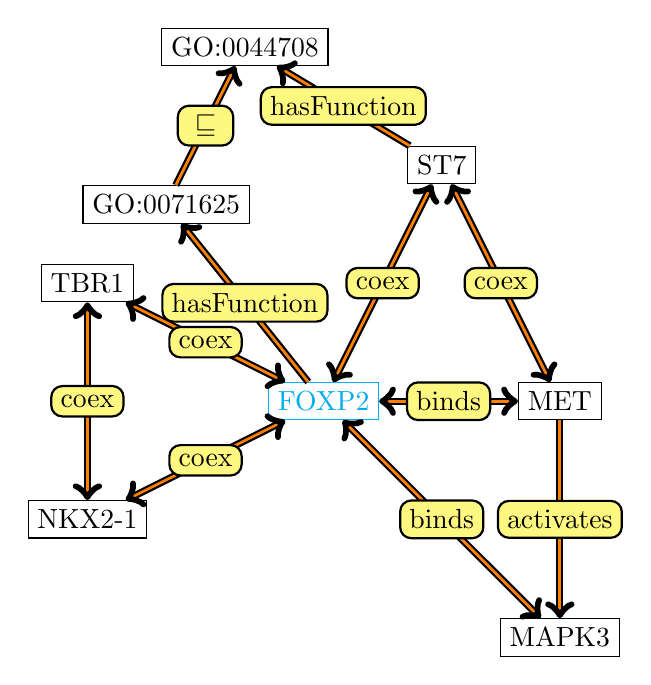
\begin{tikzpicture}
%          \SetUpEdge[lw = 1pt, color = black]
          \GraphInit[vstyle=Shade]
          \tikzset{
            LabelStyle/.style = { rectangle, rounded corners, draw,
              minimum width = 2em, fill = yellow!50,
              text = black },
            VertexStyle/.append style = { inner sep=5pt,
              font = \Large\bfseries},
            EdgeStyle/.append style = {->} }
          
          \SetGraphUnit{5}
          % \tikzset{VertexStyle/.append style={fill}}
          % \tikzset{EdgeStyle/.style={->}}
          \node[draw, color=cyan] (FOXP2) at (0,0) {FOXP2};
          \node[draw] (MET) at (3,0) {MET};
          \node[draw] (ST7) at (1.5,3) {ST7};
          \node[draw] (MAPK3) at (3,-3) {MAPK3};
          \node[draw] (GO0071625) at (-2,2.5) {GO:0071625};
          \node[draw] (GO0044708) at (-1,4.5) {GO:0044708};
          \node[draw] (TBR1) at (-3,1.5) {TBR1};
          \node[draw] (NKX2-1) at (-3,-1.5) {NKX2-1};
          \begin{scope}[/tikz/handle active characters in nodes=false]
          \Edge[label=activates](MET)(MAPK3)
          \Edge[label=hasFunction](FOXP2)(GO0071625)
          \Edge[label=hasFunction](ST7)(GO0044708)
          \Edge[label=$\sqsubseteq$](GO0071625)(GO0044708)

          \tikzset{EdgeStyle/.append style={<->}}
          \Edge[label=binds](FOXP2)(MET)
          \Edge[label=binds](FOXP2)(MAPK3)
          \Edge[label=coex](FOXP2)(TBR1)
          \Edge[label=coex](FOXP2)(NKX2-1)
          \Edge[label=coex](FOXP2)(ST7)
          \Edge[label=coex](MET)(ST7)
          \Edge[label=coex](NKX2-1)(TBR1)
          \end{scope}
          % \tikzset{EdgeStyle/.style={->}}
          % \Edge[label=hf](FOXP2)(GO0044708)
          % \draw[label=binds] (FOXP2) to (MET);
          % \Edge[label=binds](FOXP2)(MET)
          % \Edge[label=activates](MET)(MAPK3)
          % \Edge[label=coexpressed-with](FOXP2)(FOXP4)
          
        \end{tikzpicture}
      }
    \end{column}
    \begin{column}{.4\textwidth}
      \begin{itemize}
      \item precompute the deductive closure:
      \item for all $\phi$: if $\mathcal{KG} \models \phi$, add $\phi$
        to $\mathcal{KG}$
      \end{itemize}
    \end{column}
  \end{columns}
      
\end{frame}

\begin{frame}
  \frametitle{Random walks}
%  \frametitle{Neuro-symbolic feature learning}
  \begin{columns}
    \begin{column}{.6\textwidth}
      \resizebox{1\textwidth}{!}{%
        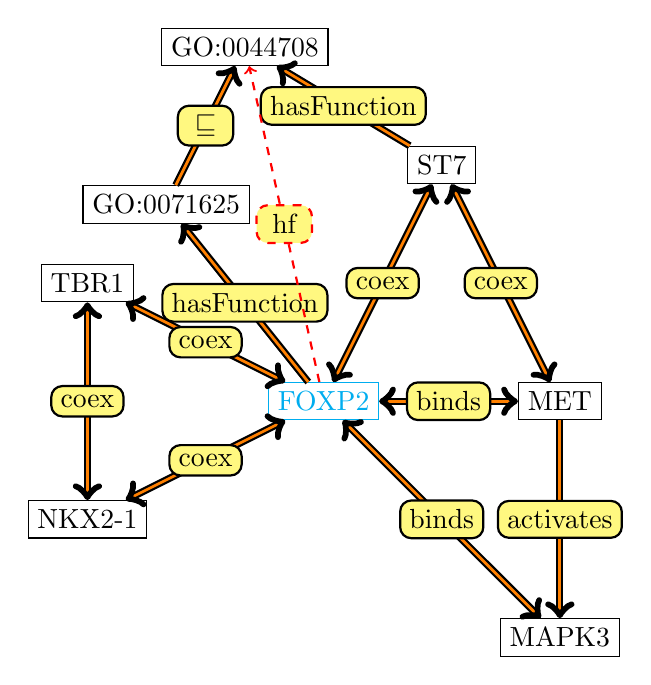
\begin{tikzpicture}
%          \SetUpEdge[lw = 1pt, color = black]
          \GraphInit[vstyle=Shade]
          \tikzset{
            LabelStyle/.style = { rectangle, rounded corners, draw,
              minimum width = 2em, fill = yellow!50,
              text = black },
            VertexStyle/.append style = { inner sep=5pt,
              font = \Large\bfseries},
            EdgeStyle/.append style = {->} }
          
          \SetGraphUnit{5}
          % \tikzset{VertexStyle/.append style={fill}}
          % \tikzset{EdgeStyle/.style={->}}
          \node[draw, color=cyan] (FOXP2) at (0,0) {FOXP2};
          \node[draw] (MET) at (3,0) {MET};
          \node[draw] (ST7) at (1.5,3) {ST7};
          \node[draw] (MAPK3) at (3,-3) {MAPK3};
          \node[draw] (GO0071625) at (-2,2.5) {GO:0071625};
          \node[draw] (GO0044708) at (-1,4.5) {GO:0044708};
          \node[draw] (TBR1) at (-3,1.5) {TBR1};
          \node[draw] (NKX2-1) at (-3,-1.5) {NKX2-1};
          \begin{scope}[/tikz/handle active characters in nodes=false]
          \Edge[label=activates](MET)(MAPK3)
          \Edge[label=hasFunction](FOXP2)(GO0071625)
          \Edge[label=hasFunction](ST7)(GO0044708)
          \Edge[label=$\sqsubseteq$](GO0071625)(GO0044708)

          \tikzset{EdgeStyle/.append style={<->}}
          \Edge[label=binds](FOXP2)(MET)
          \Edge[label=binds](FOXP2)(MAPK3)
          \Edge[label=coex](FOXP2)(TBR1)
          \Edge[label=coex](FOXP2)(NKX2-1)
          \Edge[label=coex](FOXP2)(ST7)
          \Edge[label=coex](MET)(ST7)
          \Edge[label=coex](NKX2-1)(TBR1)

          \tikzset{EdgeStyle/.style={->}}
          \Edge[label=hf, color=red, style=dashed](FOXP2)(GO0044708)
          \end{scope}
          % \tikzset{EdgeStyle/.style={->}}
          % \Edge[label=hf](FOXP2)(GO0044708)
          % \draw[label=binds] (FOXP2) to (MET);
          % \Edge[label=binds](FOXP2)(MET)
          % \Edge[label=activates](MET)(MAPK3)
          % \Edge[label=coexpressed-with](FOXP2)(FOXP4)
          
        \end{tikzpicture}
      }
    \end{column}
    \begin{column}{.4\textwidth}
      \begin{itemize}
      \item precompute the deductive closure:
      \item for all $\phi$: if $\mathcal{KG} \models \phi$, add $\phi$
        to $\mathcal{KG}$
      \end{itemize}
    \end{column}
  \end{columns}
\end{frame}

\begin{frame}
  \frametitle{Random walks}
%  \frametitle{Neuro-symbolic feature learning}
  \begin{columns}
    \begin{column}{.6\textwidth}
      \resizebox{1\textwidth}{!}{%
        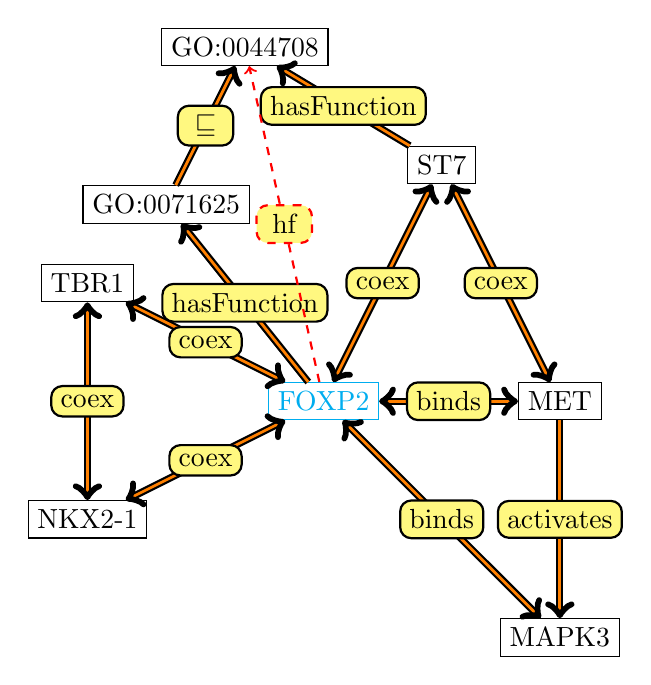
\begin{tikzpicture}
%          \SetUpEdge[lw = 1pt, color = black]
          \GraphInit[vstyle=Shade]
          \tikzset{
            LabelStyle/.style = { rectangle, rounded corners, draw,
              minimum width = 2em, fill = yellow!50,
              text = black },
            VertexStyle/.append style = { inner sep=5pt,
              font = \Large\bfseries},
            EdgeStyle/.append style = {->} }
          
          \SetGraphUnit{5}
          % \tikzset{VertexStyle/.append style={fill}}
          % \tikzset{EdgeStyle/.style={->}}
          \node[draw, color=cyan] (FOXP2) at (0,0) {FOXP2};
          \node[draw] (MET) at (3,0) {MET};
          \node[draw] (ST7) at (1.5,3) {ST7};
          \node[draw] (MAPK3) at (3,-3) {MAPK3};
          \node[draw] (GO0071625) at (-2,2.5) {GO:0071625};
          \node[draw] (GO0044708) at (-1,4.5) {GO:0044708};
          \node[draw] (TBR1) at (-3,1.5) {TBR1};
          \node[draw] (NKX2-1) at (-3,-1.5) {NKX2-1};
          \begin{scope}[/tikz/handle active characters in nodes=false]
          \Edge[label=activates](MET)(MAPK3)
          \Edge[label=hasFunction](FOXP2)(GO0071625)
          \Edge[label=hasFunction](ST7)(GO0044708)
          \Edge[label=$\sqsubseteq$](GO0071625)(GO0044708)

          \tikzset{EdgeStyle/.append style={<->}}
          \Edge[label=binds](FOXP2)(MET)
          \Edge[label=binds](FOXP2)(MAPK3)
          \Edge[label=coex](FOXP2)(TBR1)
          \Edge[label=coex](FOXP2)(NKX2-1)
          \Edge[label=coex](FOXP2)(ST7)
          \Edge[label=coex](MET)(ST7)
          \Edge[label=coex](NKX2-1)(TBR1)

          \tikzset{EdgeStyle/.style={->}}
          \Edge[label=hf, color=red, style=dashed](FOXP2)(GO0044708)
          \end{scope}
          % \draw[label=binds] (FOXP2) to (MET);
          % \Edge[label=binds](FOXP2)(MET)
          % \Edge[label=activates](MET)(MAPK3)
          % \Edge[label=coexpressed-with](FOXP2)(FOXP4)
          
        \end{tikzpicture}
      }
    \end{column}
    \begin{column}{.4\textwidth}
      \begin{itemize}
      \item Exploring the graph:
        \pause
      \item :FOXP2 :binds :MET :coex :ST7 :hasFunction GO:0044708
        \pause
      \item :FOXP2 :hasFunction GO:0071625 subClassOf GO:0044708
        \pause
      \item :FOXP2 :coex :TBR1 :coex :NKX2-1 :coex :TBR1 :coex ...
      \end{itemize}
    \end{column}
  \end{columns}
\end{frame}

\begin{frame}
  \frametitle{Word2Vec and Random Walks}
  \begin{itemize}
  \item random walks ``flatten'' a graph
    \begin{itemize}
    \item walks capture node neighborhood
    \item and generate a ``corpus''
    \end{itemize}
  \item random walks capture graph ``structure''
    \begin{itemize}
    \item in ABox and TBox
    \item hub-nodes, communities, etc.
    \item determine ``importance'' of nodes
    \end{itemize}
  \item embeddings capture co-occurrence
    \begin{itemize}
    \item similar graph neighborhood $\Rightarrow$ similar
      co-occurrence $\Rightarrow$ similar vector
    \end{itemize}
  \item embeddings generate ``feature'' vectors
    \begin{itemize}
    \item functions from symbols (words, labels) into $\Re^n$
    \end{itemize}
  \end{itemize}
\end{frame}

\begin{frame}
  \frametitle{What to do with embeddings?}
  \begin{itemize}
  \item useful for edge prediction, similarity, clustering, as feature
    vectors
    \begin{itemize}
    \item supervised: edge prediction (e.g., SVM, ANN)
      \begin{itemize}
      \item e.g.: find a function $f:\Re^n \times \Re^n \mapsto [0,1]$
        s.t. $\sqrt \frac{\sum_{t=1}^T (\hat{y_t} - y_t)^2}{T}$ (RMSE)
        is minimized for a set of true labels $y_k$
      \end{itemize}
    \item unsupervised: clustering, similarity, visualization
      \begin{itemize}
      \item cosine similarity (for L2-normalized features)
      \item Word2Vec embeddings capture similarity between co-occurrence vectors
      \end{itemize}
    \end{itemize}
  \end{itemize}
\end{frame}

% \begin{frame}
%   \frametitle{Visualizing feature vectors: dimensionality reduction}
%   \begin{itemize}
%   \item project $n$-dimensional vectors in 2D (or 3D) space
%   \item and color with some known labels
%     \begin{itemize}
%     \item high-level/general classes in an ontology work great
%     \end{itemize}
%   \item PCA or t-SNE
%   \item \url{https://lvdmaaten.github.io/tsne/}
%   \end{itemize}
% \end{frame}

% \begin{frame}
%   \frametitle{Visualizing feature vectors}
% %  \frametitle{Neuro-symbolic feature learning}
%   \centerline{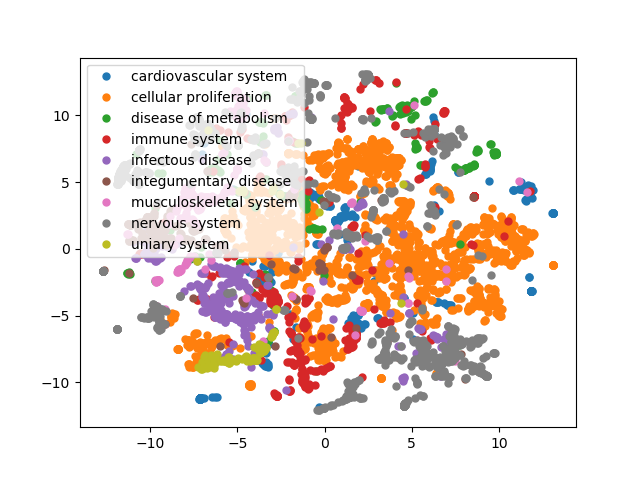
\includegraphics[width=\textwidth]{graph-tsne.png}}
% \end{frame}

% \begin{frame}
%   \frametitle{Features: supervised learning}
%   \begin{itemize}
%   \item feature vectors represent graph neighborhood of nodes
%     \begin{itemize}
%     \item adjacent nodes and edges
%     \item ontology classes (asserted \& inferred)
%     \end{itemize}
%   \item useful in supervised prediction tasks
%   \item relation prediction:
%     \begin{itemize}
%     \item input: two features vectors (from embedding function)
%     \item output: $0$ or $1$ (relation or not)
%     \item training data: positive and negative cases
%       \begin{itemize}
%       \item $R(x,y)$ and $\neg R(x,y)$
%       \item $R(x,y)$ and not provable $R(x,y)$
%       \end{itemize}
%     \end{itemize}
%   \end{itemize}
% \end{frame}

% \begin{frame}
% %  \frametitle{Random walks}
% %  \frametitle{Neuro-symbolic feature learning}
%   \frametitle{Features: supervised learning}
%   \centerline{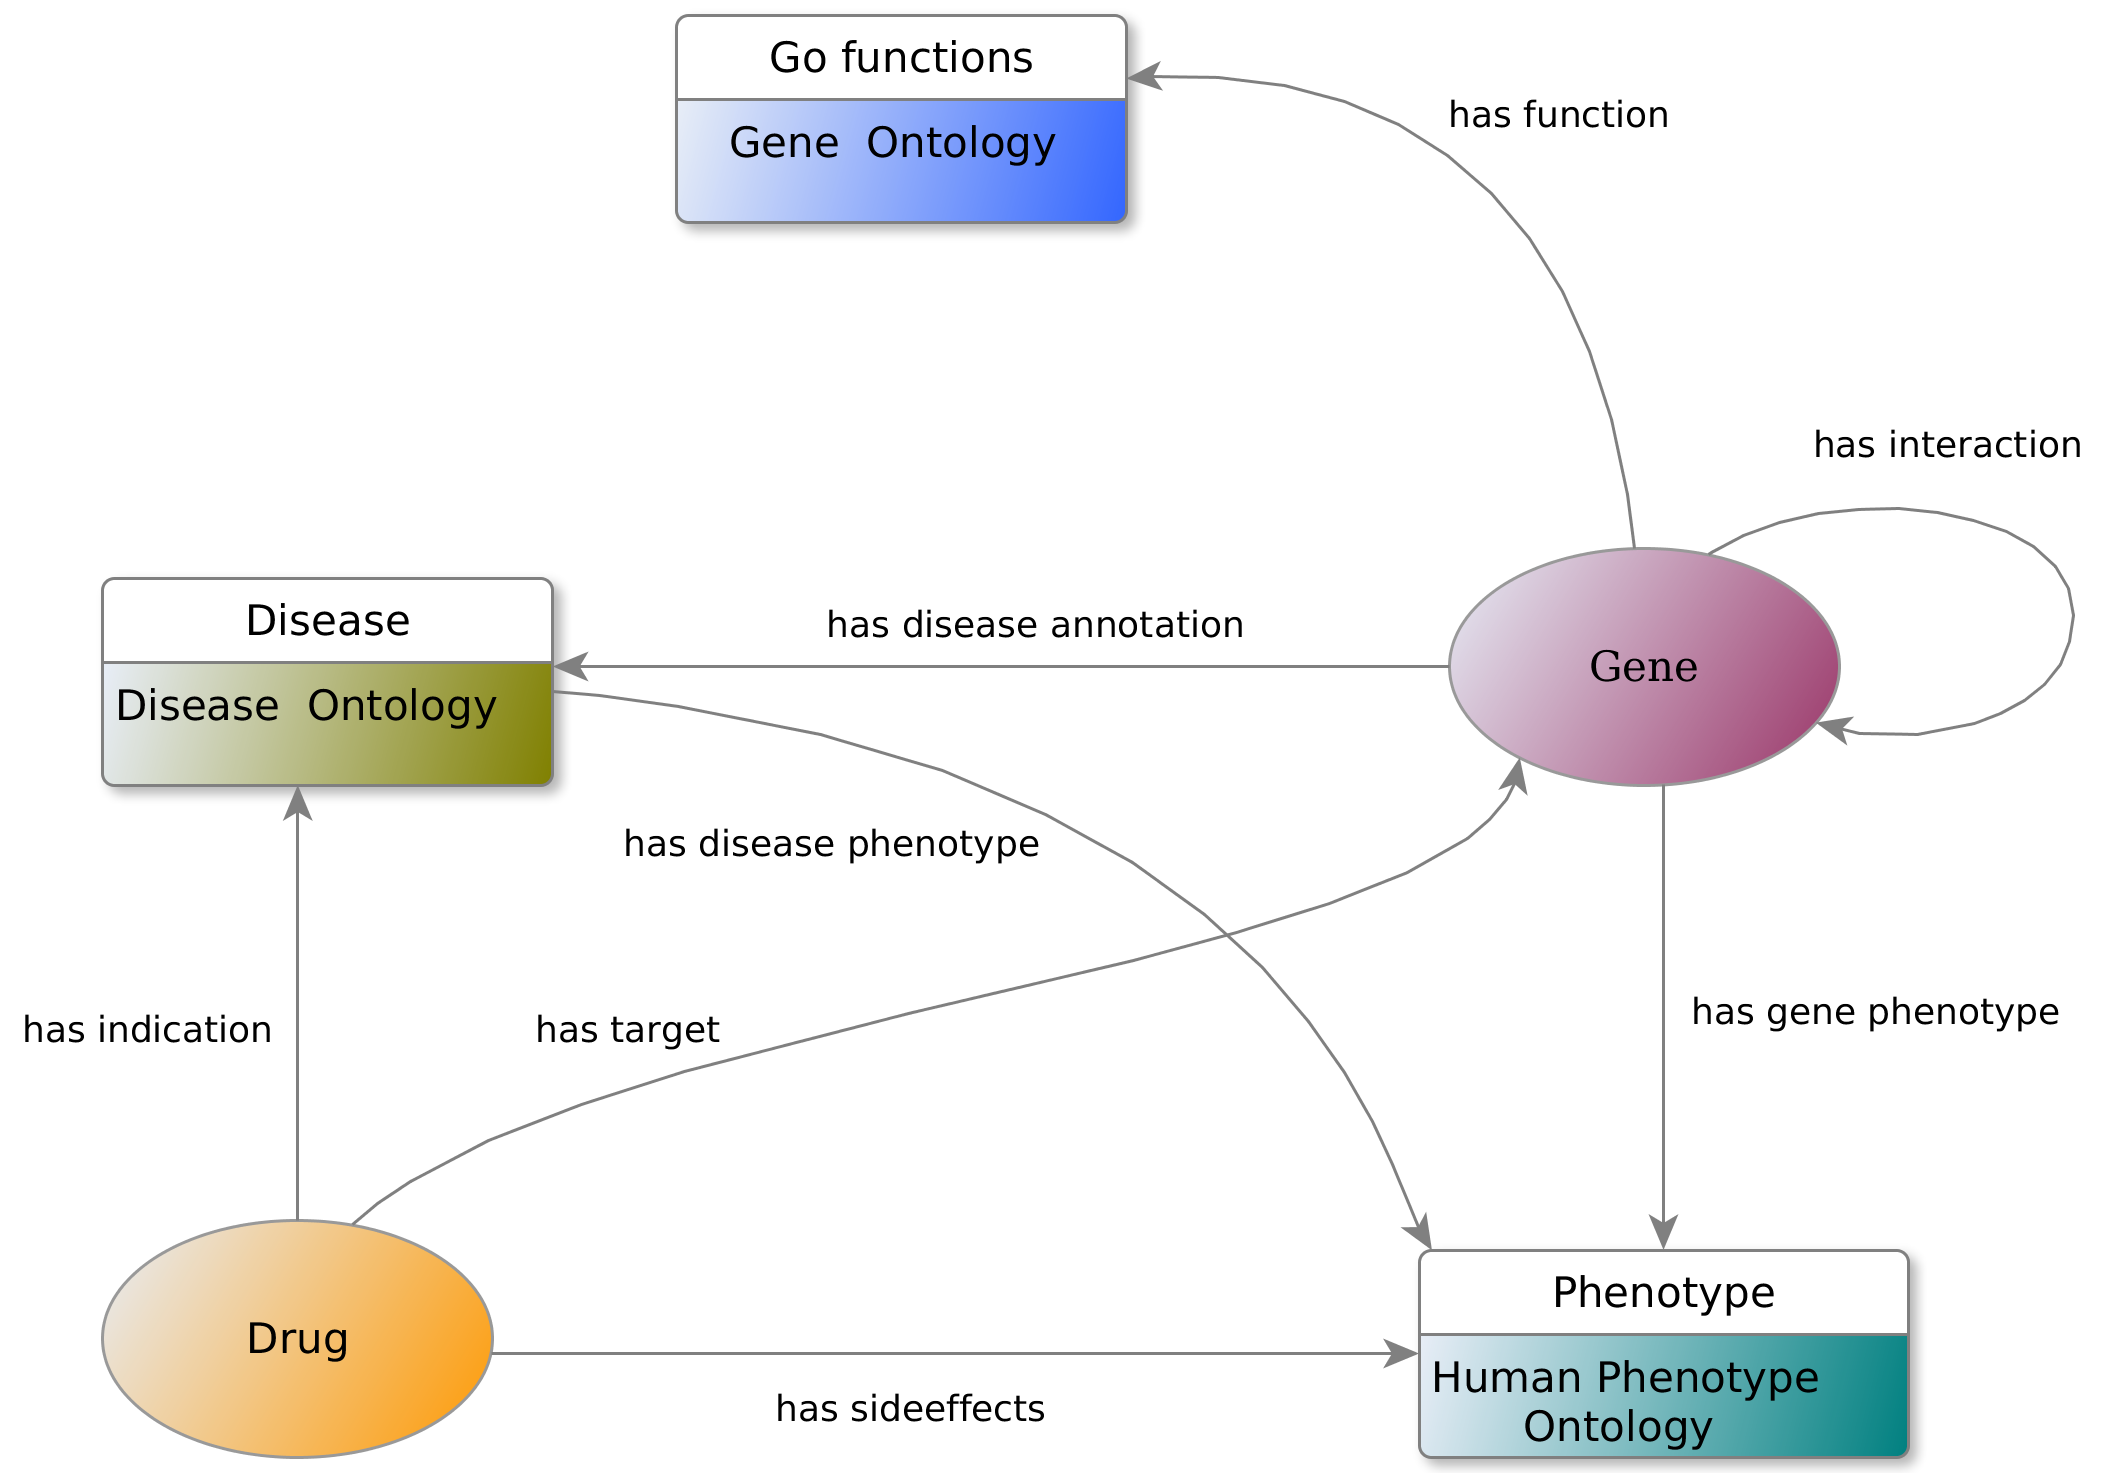
\includegraphics[width=\textwidth]{rdf-walking-datasets.png}}
% \end{frame}

% \begin{frame}
%   \frametitle{Features: supervised learning}
%   \resizebox{\textwidth}{!}{
%   \begin{tabular}{@{}lllcccc@{}}\toprule 
%       \multirow{2}{*}{Object property} 
%       & Source type & Target type &\multicolumn{2}{c}{Without reasoning}&\multicolumn{2}{c}{With reasoning}\\
%       &&& F-measure & AUC & F-measure & AUC \\
%       \midrule
%       has target & Drug & Gene/Protein & 0.94 & 0.97 & 0.94 & 0.98 \\
%       has disease annotation & Gene/Protein & Disease & 0.89 & 0.95 & 0.89 & 0.95 \\
%       has side-effect$^*$ & Drug & Phenotype & 0.86 & 0.93 & 0.87 & 0.94 \\
%       has interaction & Gene/Protein & Gene/Protein & 0.82 & 0.88 & 0.82 & 0.88\\
%       has function$^*$ & Gene/Protein & Function & 0.85 & 0.95 & 0.83 & 0.91 \\
%       has gene phenotype$^*$  & Gene/Protein & Phenotype & 0.84 & 0.91 & 0.82 & 0.90  \\
%       has indication & Drug & Disease & 0.72 & 0.79 & 0.76 & 0.83 \\
%       has disease phenotype$^*$  & Disease & Phenotype & 0.72 & 0.78 & 0.70 & 0.77 \\
%     \end{tabular}}
% \end{frame}

\begin{frame}
  \frametitle{Ontologies, graphs, and text}
    \begin{quote}
      The \only<1,2>{\underline{forkhead-box P2 (FOXP2)}}\only<3>{\underline{:FOXP2}} gene polymorphism has been
      reported to be involved in the susceptibility to schizophrenia;
      however, few studies have investigated the association between
      \only<1,2>{\underline{FOXP2}}\only<3>{\underline{:FOXP2}} gene polymorphism and clinical symptoms in schizophrenia.
    \end{quote}
  \pause
  \begin{itemize}
  \item \underline{:FOXP2} :binds :MET :coex :ST7 :hasFunction GO:0044708
  \item \underline{:FOXP2} :hasFunction GO:0071625 subClassOf GO:0044708
  \item \underline{:FOXP2} :coex :TBR1 :coex :NKX2-1 :coex :TBR1 :coex ...
  \end{itemize}
\end{frame}

% \begin{frame}
%   \frametitle{Multi-modal feature learning}
%   \centerline{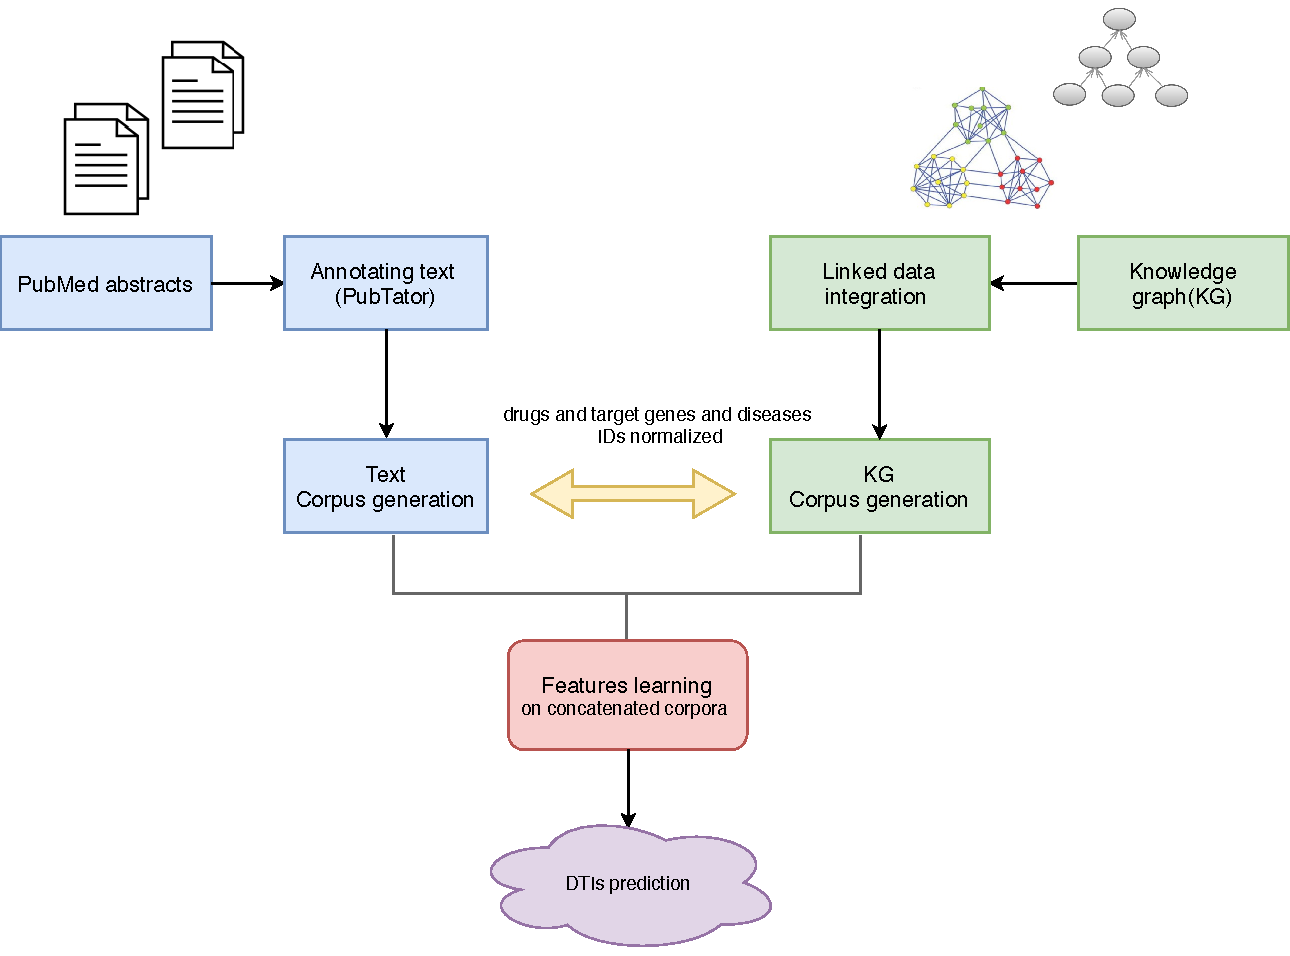
\includegraphics[width=\textwidth]{multimodal_workflow.pdf}}
% \end{frame}


% \begin{frame}
%   \frametitle{Multi-modal feature learning: drug targets and indications}
%   \centerline{
%     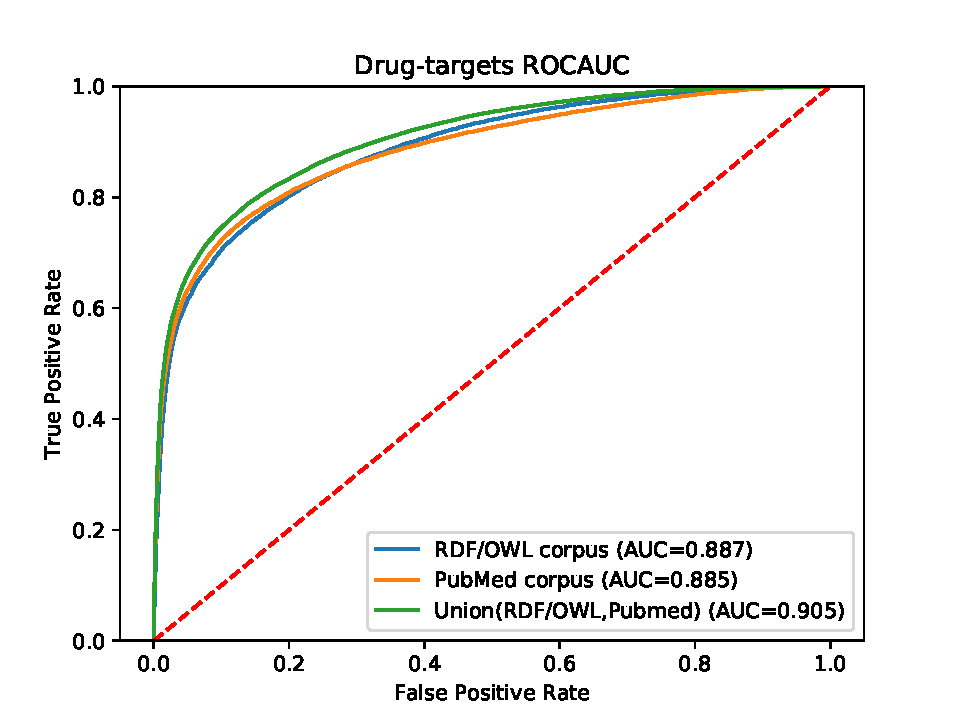
\includegraphics[width=.45\textwidth]{DTI_ANN_all.pdf}
%     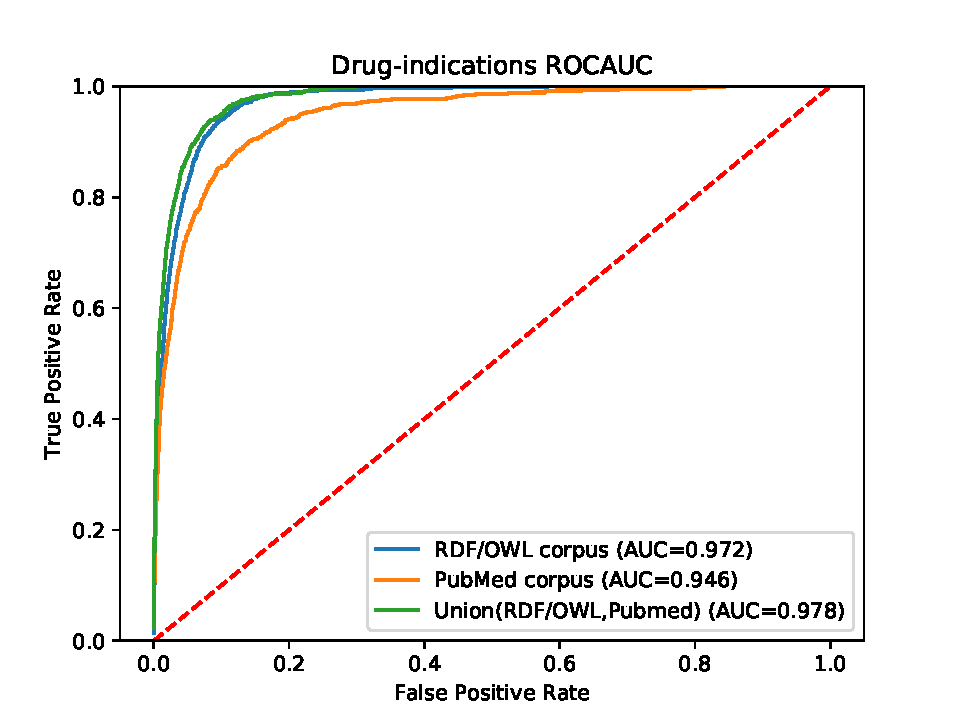
\includegraphics[width=.45\textwidth]{Ind_ANN_all.pdf}
%   }
%   \vspace{.5cm}
%   {\tiny Alshahrani \& H. Drug repurposing through
%     multi-modal learning on knowledge graphs. BioRxiv, 2018.}
% \end{frame}

\begin{frame}
  \frametitle{Tools and resources}
  \begin{itemize}
  \item RDF2Vec: random walks on RDF + Word2Vec
  \item RDF2Vec: Weisfeiler-Lehmann kernel on RDF
  \item \url{https://datalab.rwth-aachen.de/embedding/RDF2Vec/}
    \pause
  \item Walking RDF+OWL: random walks on RDF + Elk + Word2Vec
    \begin{itemize}
    \item inference
    \end{itemize}
  \item \url{https://github.com/bio-ontology-research-group/walking-rdf-and-owl}
  \end{itemize}
\end{frame}

\begin{frame}
  \frametitle{Some limitations}
  \begin{itemize}
  \item ``word''-based (Word2Vec):
    \begin{itemize}
    \item semantics is reduced to co-occurrence (in ABox/TBox
      statements)
    \item ``disjointWith'' vs. ``part-of'' vs. ``subClassOf''
    \end{itemize}
  \end{itemize}
\end{frame}

% \begin{frame}
%   \frametitle{Jupyter excercise}
%   \begin{itemize}
%   \item Open the Jupyter notebook {\tt graph.ipynb}
%   \item Follow the examples in the first part of the notebook (random
%     walks)
%   \item If you don't have a powerful CPU in your laptop (with multiple
%     cores), you may want to lower the number of iterations ({\tt
%       n\_iter}) during TSNE
%   \item some of the code will take a while to run
%     \begin{itemize}
%     \item if things are too slow, you can keep it running while we
%       continue or complete this after the tutorial
%     \end{itemize}
%   \item (some notes on parameters and hyperparameters...)
%   \end{itemize}
% \end{frame}


\subsection{Translating embeddings}
\begin{frame}
  \frametitle{Translating embeddings}
  \begin{definition}
    Let $KG = (V, E, L; \vdash)$ be a knowledge graph with a set of
    vertices $V$, a set of edges $E \subseteq V \times V$, a label
    function $L: V \cup E \mapsto Lab$ that assigns labels from a set
    of labels $Lab$ to vertices and edges, and an inference relation
    $\vdash$. A knowledge graph embedding is a function
    $f_\eta : L(V) \cup L(E) \mapsto \mathbf{R}^n$.
  \end{definition}
  \pause
  Graph as edgelist: set of $(s,p,o)$ statements\\
  \pause
  Idea: $\mu (s) + \mu (p) \approx \mu (o)$\\
  \pause
  Minimize: $\sum_t \norm{ \mu (s) + \mu (p) - \mu (o) }$ (chose your
  norm, usually L2)
\end{frame}

\begin{frame}
  \frametitle{Translating embeddings}
  \centerline{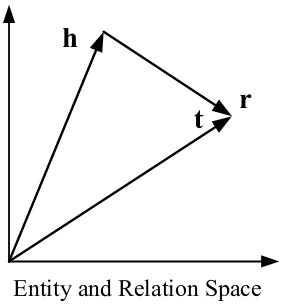
\includegraphics[width=.7\textwidth]{transe-figure.png}}
\end{frame}

\begin{frame}
  \frametitle{Translating embeddings}
  \begin{columns}
    \begin{column}{.6\textwidth}
      \resizebox{1\textwidth}{!}{%
        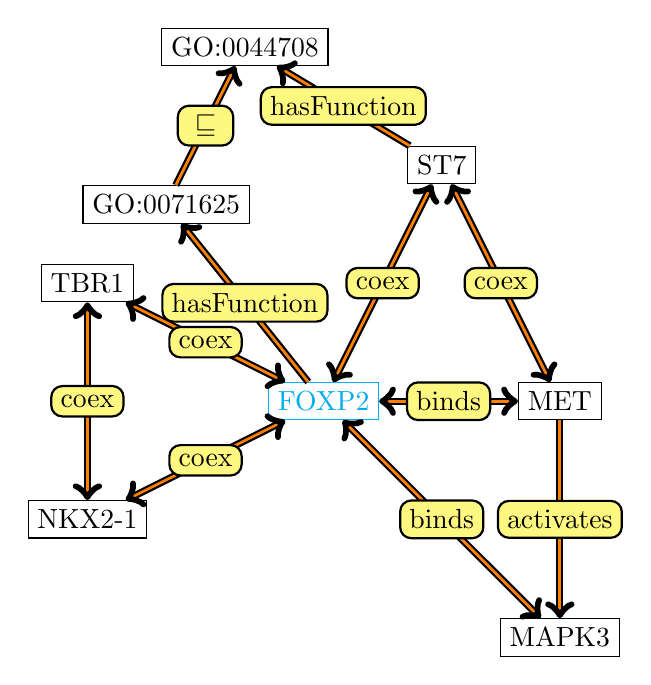
\begin{tikzpicture}
%          \SetUpEdge[lw = 1pt, color = black]
          \GraphInit[vstyle=Shade]
          \tikzset{
            LabelStyle/.style = { rectangle, rounded corners, draw,
              minimum width = 2em, fill = yellow!50,
              text = black },
            VertexStyle/.append style = { inner sep=5pt,
              font = \Large\bfseries},
            EdgeStyle/.append style = {->} }
          
          \SetGraphUnit{5}
          % \tikzset{VertexStyle/.append style={fill}}
          % \tikzset{EdgeStyle/.style={->}}
          \node[draw, color=cyan] (FOXP2) at (0,0) {FOXP2};
          \node[draw] (MET) at (3,0) {MET};
          \node[draw] (ST7) at (1.5,3) {ST7};
          \node[draw] (MAPK3) at (3,-3) {MAPK3};
          \node[draw] (GO0071625) at (-2,2.5) {GO:0071625};
          \node[draw] (GO0044708) at (-1,4.5) {GO:0044708};
          \node[draw] (TBR1) at (-3,1.5) {TBR1};
          \node[draw] (NKX2-1) at (-3,-1.5) {NKX2-1};
          \begin{scope}[/tikz/handle active characters in nodes=false]
          \Edge[label=activates](MET)(MAPK3)
          \Edge[label=hasFunction](FOXP2)(GO0071625)
          \Edge[label=hasFunction](ST7)(GO0044708)
          \Edge[label=$\sqsubseteq$](GO0071625)(GO0044708)

          \tikzset{EdgeStyle/.append style={<->}}
          \Edge[label=binds](FOXP2)(MET)
          \Edge[label=binds](FOXP2)(MAPK3)
          \Edge[label=coex](FOXP2)(TBR1)
          \Edge[label=coex](FOXP2)(NKX2-1)
          \Edge[label=coex](FOXP2)(ST7)
          \Edge[label=coex](MET)(ST7)
          \Edge[label=coex](NKX2-1)(TBR1)
          \end{scope}
          % \tikzset{EdgeStyle/.style={->}}
          % \Edge[label=hf](FOXP2)(GO0044708)
          % \draw[label=binds] (FOXP2) to (MET);
          % \Edge[label=binds](FOXP2)(MET)
          % \Edge[label=activates](MET)(MAPK3)
          % \Edge[label=coexpressed-with](FOXP2)(FOXP4)
          
        \end{tikzpicture}
      }
    \end{column}
    \begin{column}{.4\textwidth}
      \begin{itemize}
        \pause
      \item FOXP2 + binds = MET
        \pause
      \item MET + activates = MAPK3
        \pause
      \item MET + binds = FOXP2
        \pause
      \item ST7 + hasFunction = {\tt GO:0044708}
        \pause
      \item ...
      \end{itemize}
    \end{column}
  \end{columns}
\end{frame}

\begin{frame}
  \frametitle{Translating embeddings}
  \begin{columns}
    \begin{column}{.6\textwidth}
      \resizebox{1\textwidth}{!}{%
        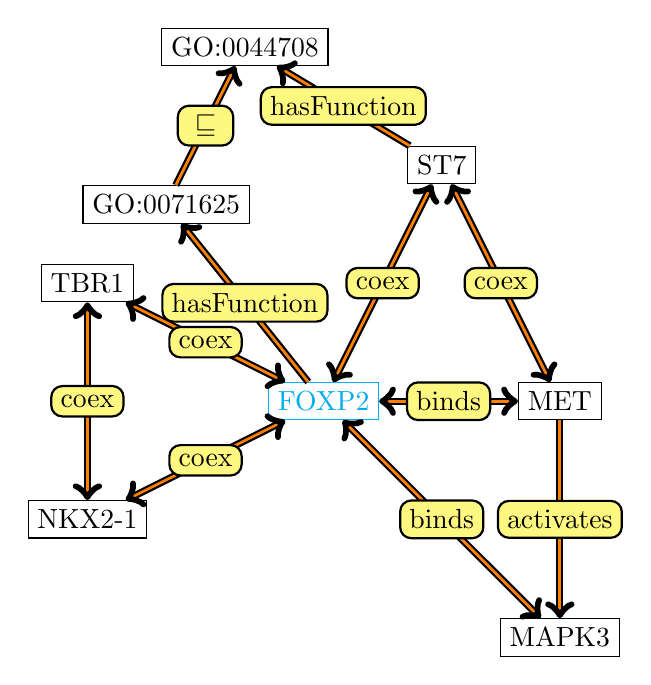
\begin{tikzpicture}
%          \SetUpEdge[lw = 1pt, color = black]
          \GraphInit[vstyle=Shade]
          \tikzset{
            LabelStyle/.style = { rectangle, rounded corners, draw,
              minimum width = 2em, fill = yellow!50,
              text = black },
            VertexStyle/.append style = { inner sep=5pt,
              font = \Large\bfseries},
            EdgeStyle/.append style = {->} }
          
          \SetGraphUnit{5}
          % \tikzset{VertexStyle/.append style={fill}}
          % \tikzset{EdgeStyle/.style={->}}
          \node[draw, color=cyan] (FOXP2) at (0,0) {FOXP2};
          \node[draw] (MET) at (3,0) {MET};
          \node[draw] (ST7) at (1.5,3) {ST7};
          \node[draw] (MAPK3) at (3,-3) {MAPK3};
          \node[draw] (GO0071625) at (-2,2.5) {GO:0071625};
          \node[draw] (GO0044708) at (-1,4.5) {GO:0044708};
          \node[draw] (TBR1) at (-3,1.5) {TBR1};
          \node[draw] (NKX2-1) at (-3,-1.5) {NKX2-1};
          \begin{scope}[/tikz/handle active characters in nodes=false]
          \Edge[label=activates](MET)(MAPK3)
          \Edge[label=hasFunction](FOXP2)(GO0071625)
          \Edge[label=hasFunction](ST7)(GO0044708)
          \Edge[label=$\sqsubseteq$](GO0071625)(GO0044708)

          \tikzset{EdgeStyle/.append style={<->}}
          \Edge[label=binds](FOXP2)(MET)
          \Edge[label=binds](FOXP2)(MAPK3)
          \Edge[label=coex](FOXP2)(TBR1)
          \Edge[label=coex](FOXP2)(NKX2-1)
          \Edge[label=coex](FOXP2)(ST7)
          \Edge[label=coex](MET)(ST7)
          \Edge[label=coex](NKX2-1)(TBR1)
          \end{scope}
          % \tikzset{EdgeStyle/.style={->}}
          % \Edge[label=hf](FOXP2)(GO0044708)
          % \draw[label=binds] (FOXP2) to (MET);
          % \Edge[label=binds](FOXP2)(MET)
          % \Edge[label=activates](MET)(MAPK3)
          % \Edge[label=coexpressed-with](FOXP2)(FOXP4)
          
        \end{tikzpicture}
      }
    \end{column}
    \begin{column}{.4\textwidth}
      \begin{itemize}
      \item FOXP2 + binds - MET = 0
      \item MAP + activates - MAPK3 = 0
      \item MET + binds - FOXP2 = 0
      \item ST7 + hasFunction - {\tt GO:0044708} = 0
      \item ...
      \end{itemize}
    \end{column}
  \end{columns}
\end{frame}

% \begin{frame}
%   \frametitle{Translating embeddings}
%   \centerline{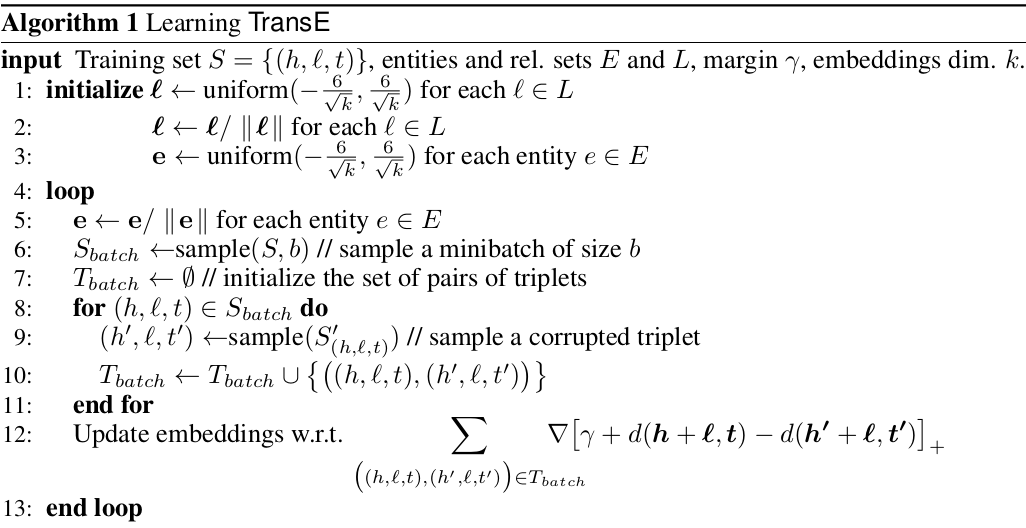
\includegraphics[width=1\textwidth]{transe-algorithm.png}}

%   {\tiny Bordes et al. (2013). Translating Embeddings for
%     Modeling Multi-relational Data.}
% \end{frame}

\begin{frame}
  \frametitle{Some properties of TransE}
  \begin{itemize}
  \item graph-based
    \begin{itemize}
    \item works well on RDF graphs
    \item and ontology graphs
    \end{itemize}
  \item 1:1 relations only
    \begin{itemize}
    \item not suitable for hierarchies (1-N relations)
    \item not suitable for N-N relations
    \item no transitive, symmetric, reflexive relations
    \end{itemize}
  \end{itemize}
\end{frame}

\begin{frame}
  \frametitle{Translating embeddings}
  \centerline{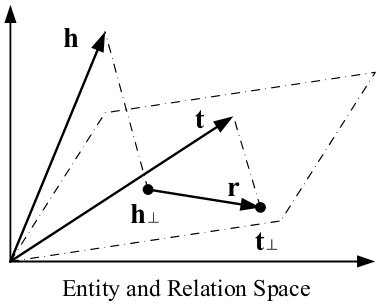
\includegraphics[width=.7\textwidth]{transh-figure.png}}
\end{frame}

\begin{frame}
  \frametitle{Translating embeddings}
  \centerline{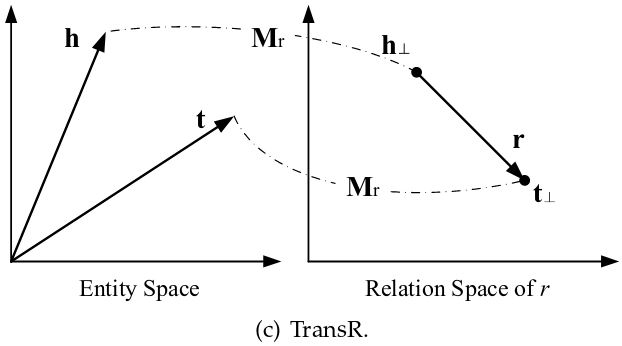
\includegraphics[width=.7\textwidth]{transr-figure.png}}
\end{frame}

% \begin{frame}
%   \frametitle{Translating embeddings}
%   \centerline{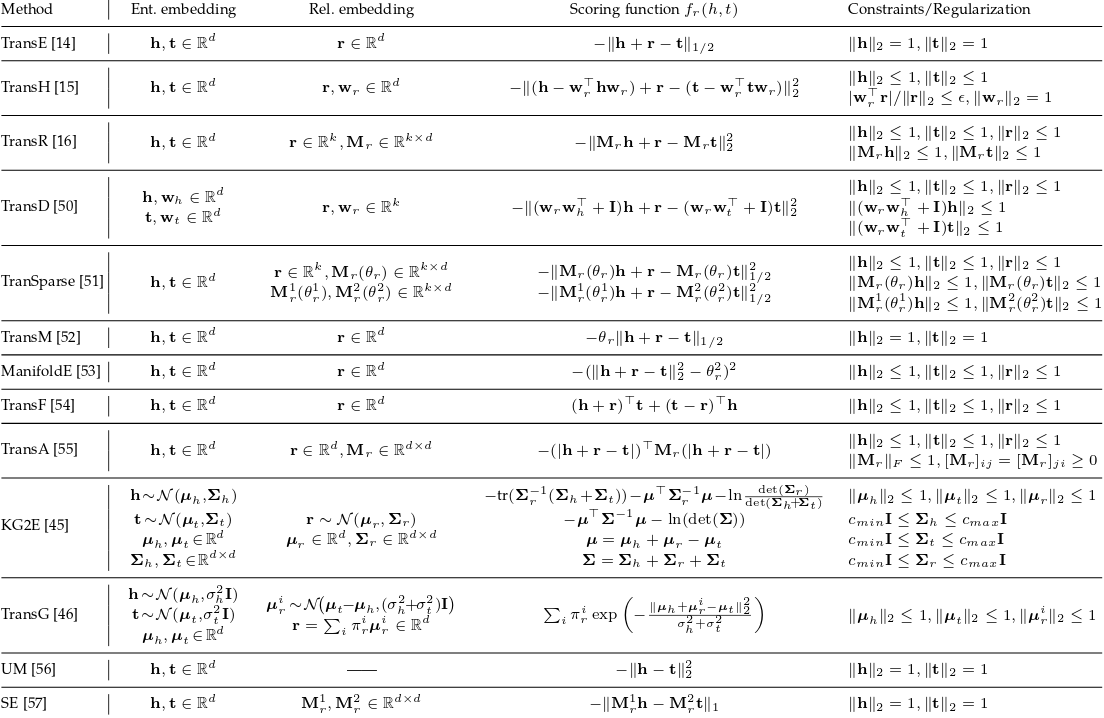
\includegraphics[width=\textwidth]{loss-functions-kg.png}}
%   {\tiny Wang et al. Knowledge Graph Embedding: A Survey ofApproaches and Applications.}
% \end{frame}

\begin{frame}
  \frametitle{PyKEEN}
  \begin{itemize}
  \item Python package to generate knowledge graph embeddings
  \item supports many different graph embedding types: TransE, TransR,
    TransD, RESCAL, etc.
  \item hyperparameter optimization (``HPO'') and evaluation included
  \item \url{https://github.com/SmartDataAnalytics/PyKEEN}
  \end{itemize}
\end{frame}

\begin{frame}
  \frametitle{Some limitations}
  \begin{itemize}
  \item graph-based (same as random walks):
    \begin{itemize}
    \item ontologies are not graphs!
    \item converting ontologies to graphs loses information
    \item no axioms, no definitions
    \end{itemize}
  \item (this also holds for Graph Convolutional Networks, which are
    not covered here)
  \end{itemize}
\end{frame}

% \begin{frame}
%   \frametitle{Jupyter excercise}
%   \begin{itemize}
%   \item run the TransE part of {\tt graph.ipynb}
%   \item again: this may take a while
%   \item you can also explore
%     \url{https://github.com/SmartDataAnalytics/PyKEEN}
%   \item try to expand the notebook to predict ``new'' relations
%     % \begin{itemize}
%     % \item using numpy directly, or PyKEEN's predictions methods
%     % \end{itemize}
%   % \item Change the TSNE to work only on enzymes (don't include the GO
%   %   classes, etc.)
%   \end{itemize}
% \end{frame}


\subsection{Model-theoretic approaches}

\begin{frame}
  \frametitle{How to overcome the semantic gap?}
  \begin{itemize}
  \item none of the models discussed above are truly ``semantic''
    \begin{itemize}
    \item all syntactic
    \item graph-based or based on axioms
    \end{itemize}
    \pause
  \item what do we actually mean by ``semantics''?
    \begin{itemize}
    \pause
    \item formal definition of ``truth'' relies on ``models''
    \pause
    \item universal algebra over formal languages (with signature
      $\Sigma$)
    \end{itemize}
  \end{itemize}
\end{frame}

\begin{frame}
  \frametitle{Description Logic EL++}
  \centering
  \resizebox{.8\textwidth}{!}{
    
    \begin{tabular}{|p{1.7cm}|c|p{3.7cm}|}
      \hline
      {\bf} Name & Syntax & Semantics \\
      \hline
      top & $\top$ & $\Delta^{\mathcal{I}}$ \\
    \hline
    bottom & $\bot$ & $\emptyset$ \\
    \hline
    nominal & $\{ a \} $ & $\{ a^{\mathcal{I}} \}$ \\
    \hline
    conjunction & $C \sqcap D$ & $ C^{\mathcal{I}} \cap
                                 D^{\mathcal{I}}$ \\
    \hline
    existential restriction & $\exists r.C$ & $ \{ x \in
                                              \Delta^{\mathcal{I}} |
                                              \exists y \in
                                              \Delta^{\mathcal{I}} :
                                              (x,y) \in
                                              r^{\mathcal{I}} \land y
                                              \in C^{\mathcal{I}} \} $
    \\
    \hline
    generalized concept inclusion & $C \sqsubseteq D$ &
                                                        $C^{\mathcal{I}}
                                                        \subseteq
                                                        D^{\mathcal{I}}$
    \\
    \hline
    role inclusion & $r_1 \circ ... \circ r_n \sqsubseteq r$ &
                                                               $r_1^{\mathcal{I}}
                                                               \circ
                                                               ... \circ
                                                               r_n^{\mathcal{I}}
                                                               \subseteq
                                                               r^{\mathcal{I}}$
    \\
    \hline
    
  \end{tabular}
}
\end{frame}

\begin{frame}
  \frametitle{Models}
  \begin{itemize}
  \item Interpretations and $\Sigma$-structures
  \item Model $\mathfrak{A}$ of a formula $\phi$: $\phi$ is true in
    $\mathfrak{A}$ ($\mathfrak{A} \models \phi$) 
  \item Theory $T$: set of formulas
  \item $\mathfrak{A}$ is a model of $T$ if $\mathfrak{A}$ is a model
    of all formulas in $T$
  \item Ontologies are (special kinds of) theories
  \end{itemize}
\end{frame}

\begin{frame}
  \frametitle{EL Embeddings}
  \begin{itemize}
  \item given a theory/ontology $T$ with signature $\Sigma(T)$
  \item aim: find $f_e: \Sigma(T) \mapsto \Re^n$ s.t. $f_e(\Sigma(T))$
    is a model of $T$ ($f_e(\Sigma(T)) \models T$)
    \pause
  \item more general: find an algorithm that maps symbols (signatures)
    into $\Re^n$ so that the {\em semantics} of the symbol (expressed
    through axioms and explicit in model structures) is preserved
    \begin{itemize}
    \item or: the embedding function {\em is} an interpretation function
    \end{itemize}

    \pause
  \item any consistent \el  theory has infinite models
    \pause
  \item any consistent \el  theory has models in $\mathbb{R}^n$
    (Loewenheim-Skolem, upwards; compactness)
  \end{itemize}
\end{frame}

\begin{frame}
  \frametitle{Key idea}
  \begin{itemize}
  \item for all $r \in \Sigma(T)$ and $C \in \Sigma(T)$, define
    $f_e(r)$ and $f_e(C)$
  \item $f_e(C)$ maps to points in an open $n$-ball such that
    $f_e(C) = C^{\mathcal{I}}$:
    $C^{\mathcal{I}} = \{ x \in \mathbb{R}^n | \norm{f_e(C) - x} <
    r_e(C) \}$
    \begin{itemize}
    \item these are the {\em extension} of a class in $\Re^n$
    \end{itemize}
  \item $f_e(r)$ maps a binary relation $r$ to a vector such that
    % the set of tuples ($\mathbb{R}^n \times \mathbb{R}^n$) with
    % $f_e(r) = r^{\mathcal{I}}$:
    $r^{\mathcal{I}} = \{ (x,y) | x + f_e(r) = y \}$
    \begin{itemize}
    \item that's the TransE property for {\em individuals}
    \end{itemize}
  \item use the axioms in $T$ as constraints
  \end{itemize}
\end{frame}

\begin{frame}
  \frametitle{Algorithm}
  \begin{itemize}
  \item normalize the theory:
    \begin{itemize}
    \item every \el theory can be expressed using four normal forms
      (Baader et al., 2005)
    \end{itemize}
  \item eliminate the ABox: replace each individual symbol with a
    singleton class: $a$ becomes $\{a\}$
  \item rewrite relation assertions $r(a,b)$ and class
    assertions $C(a)$ as $\{ a \} \sqsubseteq \exists r.\{ b \}$ and
    $\{ a \} \sqsubseteq C$
    \begin{itemize}
    \item something to remember for the next class-vs-instance discussion?
    \end{itemize}
  \item normalization rules to generate:
    \begin{itemize}
    \item $C \sqsubseteq D$
    \item $C \sqcap D \sqsubseteq E$
    \item $C \sqsubseteq \exists R.D$
    \item $\exists R.C \sqsubseteq D$
    \end{itemize}
  \end{itemize}
\end{frame}

\begin{frame}
  \frametitle{Algorithm: loss functions}
  \begin{equation}
    \label{eqn:nf1}
    \begin{split}
      & loss_{C \sqsubseteq D}(c,d) = \\
      & \max(0, \norm{f_\eta(c) - f_\eta(d)} + r_\eta(c) - r_\eta(d) - \gamma) \\
      & + |\norm{f_\eta(c)} - 1| + |\norm{f_\eta(d)} - 1|
    \end{split}
  \end{equation}
\end{frame}

\begin{frame}
  \frametitle{Algorithm: loss functions}
  Let
  $h=\frac{r_\eta(c)^2-r_\eta(d)^2+\norm{f_\eta(c) -
      f_\eta(d)}^2}{2\norm{f_\eta(c) - f_\eta(d)}}$, then the center and
  radius of the smallest $n$-ball containing the intersection of
  $\eta(C)$ and $\eta(D)$ are
  $f_\eta(c)+\frac{h}{\norm{f_\eta(c) -
      f_\eta(d)}}(f_\eta(d)-f_\eta(c))$ and $\sqrt{r_\eta(c)^2-h^2}$.
\end{frame}

\begin{frame}
  \frametitle{Algorithm: loss functions}
  \begin{equation}
    \label{eqn:nf3}
    \begin{split}
      & loss_{C \sqsubseteq \exists R.D}(c,d,r) = \\
      & \max(0, \norm{f_\eta(c) + f_\eta(r) - f_\eta(d)}  + r_\eta(c) - r_\eta(d) - \gamma) \\
      & + |\norm{f_\eta(c)} - 1| + |\norm{f_\eta(d)} - 1|
    \end{split}
  \end{equation}
\end{frame}

\begin{frame}
  \frametitle{Algorithm: loss functions}
  \begin{equation}
    \label{eqn:nf4}
    \begin{split}
      & loss_{\exists R.C \sqsubseteq D}(c,d,r) = \\
      & \max(0, \norm{f_\eta(c) - f_\eta(r) - f_\eta(d)} - r_\eta(c) - r_\eta(d) - \gamma) \\
      & + |\norm{f_\eta(c)} - 1| + |\norm{f_\eta(d)} - 1|
    \end{split}
  \end{equation}
\end{frame}

\begin{frame}
  \frametitle{Algorithm: loss functions}
  \begin{equation}
    \label{eqn:disjoint}
    \begin{split} 
      &loss_{C \sqcap D \sqsubseteq \bot}(c,d,e) = \\
      & \max(0, r_\eta(c) + r_\eta(d) - \norm{f_\eta(c) - f_\eta(d)} + \gamma) \\
      & + |\norm{f_\eta(c)} - 1| + |\norm{f_\eta(d)} - 1|
    \end{split}
  \end{equation}
\end{frame}

\begin{frame}
  \frametitle{Algorithm: loss functions}
  \centerline{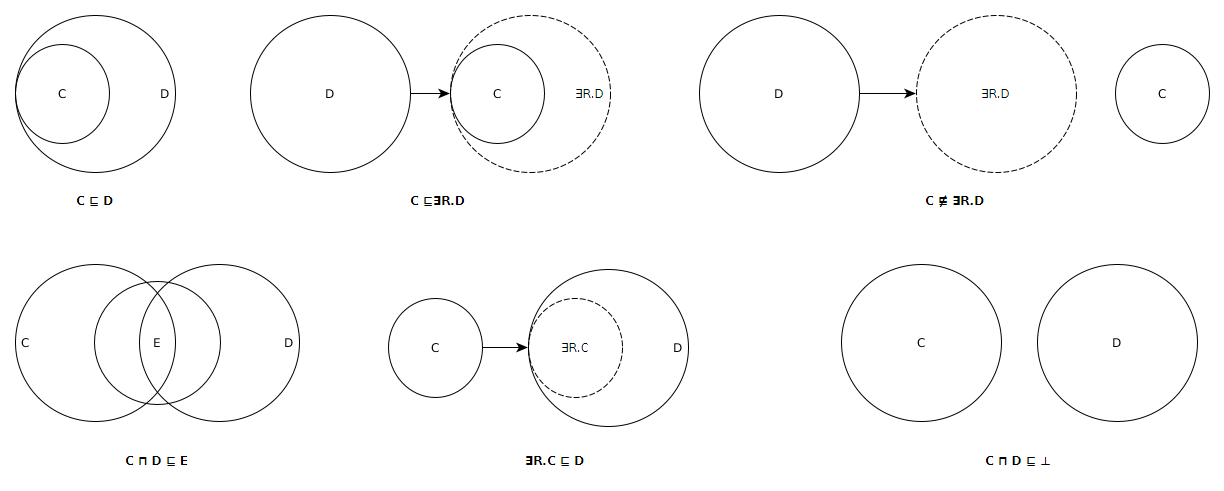
\includegraphics[width=1\textwidth]{ellosses.png}}
\end{frame}

\begin{frame}
  \frametitle{EL Embeddings}
  \begin{eqnarray}
    & Male & \sqsubseteq Person \\
    & Female & \sqsubseteq Person \\
    & Father & \sqsubseteq Male \\
    & Mother & \sqsubseteq Female \\
    & Father & \sqsubseteq Parent \\
    & Mother & \sqsubseteq Parent \\
    & Female \sqcap Male & \sqsubseteq \bot \\
    & Female \sqcap Parent & \sqsubseteq Mother \\
    & Male \sqcap Parent & \sqsubseteq Father \\
    & \exists hasChild.Person & \sqsubseteq Parent \\
    & Parent & \sqsubseteq Person \\
    & Parent & \sqsubseteq \exists hasChild.\top
               \label{famlast}
               % & Person & \sqsubseteq \top
  \end{eqnarray}
\end{frame}

\begin{frame}
  \frametitle{EL Embeddings}
  \centerline{\animategraphics[loop,controls,width=.7\textwidth]{12}{embeds-frame-}{0}{99}}
  \begin{itemize}
  \item model with $\Delta = R^n$
  \item support quantifiers, negation, conjunction,...
  \end{itemize}
\end{frame}


\end{document}

%%% Local Variables:
%%% mode: latex
%%% TeX-master: t
%%% End:
